\chapter{RFD and MRAI Interaction}
\label{cha:bgp_rfd_vs_mrai}

\fxfatal{Da rielaborare}

During \Cref{cha:bgp_mrai_experiments} I studied how \ac{MRAI} can influence
the network performances and how different factor can influence it.
Thanks to \ac{MRAI} is possible to compress the input messages choosing the best
alternative among multiple possibilities and transmitting only it as output.
I showed that the strategy is a key factor of the performances, preventing or
mitigating the \textit{Path Exploration} problem.

In \Cref{cha:bgp_rfd} I showed that \ac{RFD} can highly impact the performances,
preventing huge messages storms paying a high price in terms of convergence time.
I presented different \ac{RFD} strategies that reacts in different ways to
different signals.
The \ac{RFD} parameters play also a central role in the time required by a node
to converge because of the decay function and the reuse threshold.
This two parameters could make a route be available in less time, and by consequence,
the node would converge faster.

The hypothesis behind this study is that there is actually an interaction between
those two mechanisms.
This hypothesis is sustained by the fact that both actively act to reduce the
noise in the network and that both relies on the messages received.

In the following sections I am going to prove that an interaction exists and that \ac{MRAI}
plays a more fundamental role than \ac{RFD}.
The variation of \ac{MRAI} can provoke huge changes in the behaviour of \ac{RFD}
because the prevention of multiple messages could make the difference between
a suppression and not.
Also, \ac{RFD} could be the root cause for multiple \ac{MRAI} sessions, when
a route become available again it could trigger the distribution of multiple
messages that travels among the network.

\section{MRAI effects on toy topologies}
\label{sec:bgp_rfd_toy}

%I firstly studied \ac{RFD} on toy topologies, to see the effects of it in small
%networks, like I did in \Cref{sec:bgp_mrai_clique}.
%As a graph, I used a clique of dimension \num{10}, the source of the signalling
%is connected to the node \num{0} while the node \num{5} act as unique servicer
%for the node $x$.
%The node \num{5} won't be able to share information to node $x$ because of \ac{RFD}.
%Node $x$ would have to wait until the \ac{RFD} value of \num{5} fell below
%the reuse threshold in order to be able to converge.
%
%The parameters used for \ac{RFD} are the default \textit{CISCO} parameters,
%showed in table \Cref{tbl:cisco_rfd} and are going to be used by
%all the nodes.

%\begin{table}[h]
%	\begin{center}
	\begin{tabular}{ || m{5cm}| m{2cm} || } 
	\hline
	Parameter & Value \\ 
	\hline \hline
	withdrawal penalty & 1.0 \\
	\hline
    re-advertisement penalty & 0.0 \\
	\hline
    attribute change penalty & 1.0 \\
	\hline
    suppress threshold & 2.0 \\
	\hline
    half-life (min) & 15 (900s) \\
	\hline
    Reuse Threshold & 0.75 \\
	\hline
    Max Suppress Time (min.) & 60 (3600s) \\
	\hline
	\end{tabular}
\end{center}

%	\caption{Cisco default \ac{RFD} parameters}
%	\label{tbl:cisco_rfd}
%\end{table}

%The parameters of the environment are in \Cref{tbl:clique_rfd_params}.
%
%\begin{table}[h]
%	\begin{center}
	\begin{tabular}{ || m{4cm}| m{8cm} || } 
	\hline
	Property & Value \\ 
	\hline \hline
	Seeds & $[1, 10]$ \\ 
	\hline
	Signaling & \q{AWAWAWA} \\
	\hline
		Withdraws delay & Constant distribution of \SI{300}{\second} \\ 
	\hline
	Announcement delay & constant distribution of \SI{300}{\second} \\ 
	\hline
		MRAI & $[0, 120]$ \\
	\hline
	Link delay & Uniform distribution between \SI{0.012}{\second} and \SI{3}{\second} \\
	\hline
	\end{tabular}
\end{center}

%	\caption{Environment parameters used for the experiments on \ac{RFD}
%		with the clique graph}
%	\label{tbl:clique_rfd_params}
%\end{table}
%
%Messages in the signal are delayed by \SI{300}{\second} for two reasons:
%\begin{itemize}
%    \item We don't want that \ac{MRAI} compress parts of the signal;
%	\item I'm trying to simulate one of the possible behaviours tat triggers a
%		\ac{RFD} suppression, the human faulty reconfiguration of the node.
%\end{itemize}
%
%The signal contain \num{3} flaps, the first one is hypothetically attributed
%to a configuration that doesn't work properly, the second one is caused by a
%buggy correction of the configuration and the last one by the introduction of a
%correct configuration.
%
%The \ac{MRAI} strategy used in all the experiments is the \textit{fixed} one.

In \Cref{sec:rfd_toy_topologies} is presented a studied that uses a clique
network as graph with a fixed \ac{MRAI} of \SI{30}{\second} and the \ac{RFD}
configured like the legacy version descried in~\cite{rfc2439}.
I have then executed again those experiments with the same toy topology and the
same \ac{RFD} filter with multiple \ac{MRAI} values.
The strategy used is alway the \textit{Fixed} one, so every link have the same
value of the others.
\ac{MRAI} goes from \SI{0}{\second} up to \SI{120}{\second}.
The results are presented in \Cref{fig:clique_evolution_rfd_vs_noRFD}.

\begin{figure}[h]
     \centering
     \begin{subfigure}[b]{0.49\textwidth}
         \centering
		 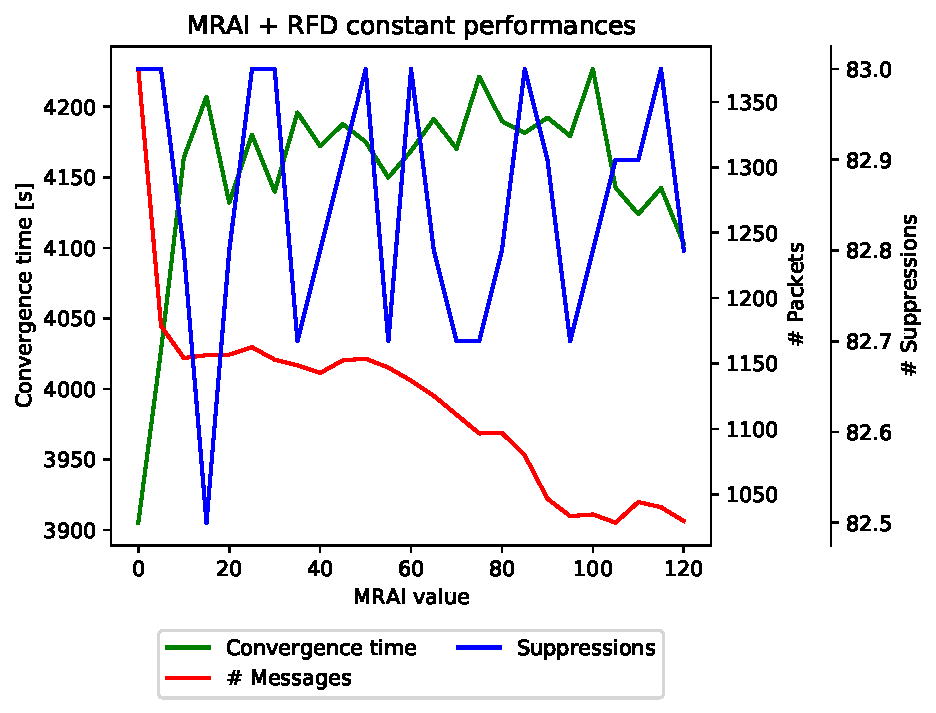
\includegraphics[width=\textwidth]{images/RFD/clique/cisco_clique10_RFD-constant_mrai_rfd_evolution.pdf}
		 \caption{Network performances with the standard cisco \ac{RFD}}
		 \label{fig:clique_evolution_rfd}
     \end{subfigure}
     \hfill
     \begin{subfigure}[b]{0.49\textwidth}
         \centering
         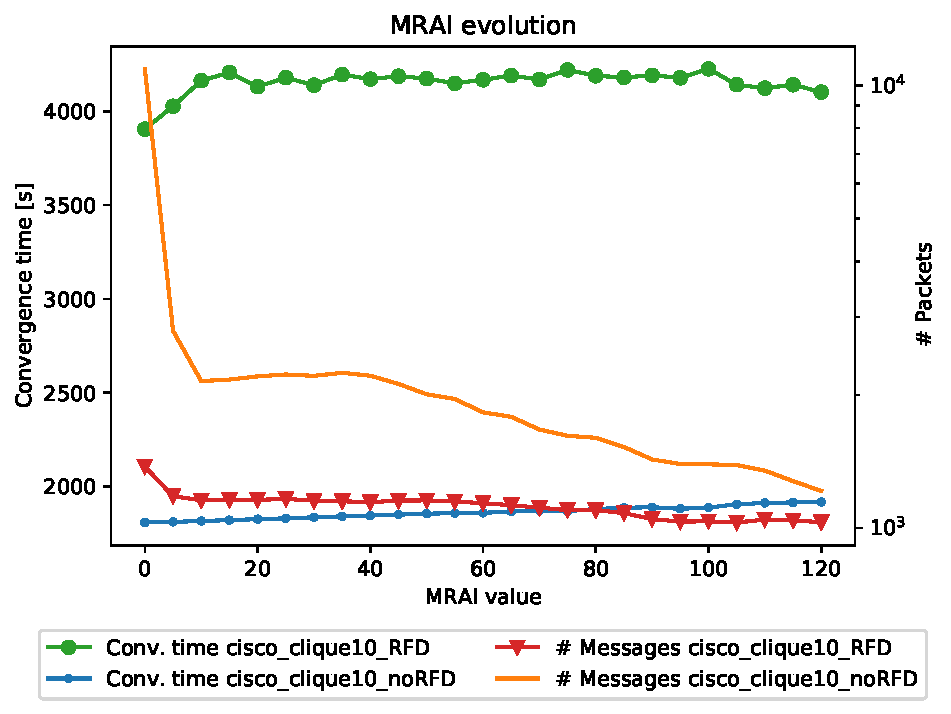
\includegraphics[width=\textwidth]{images/RFD/clique/cisco_clique10_comparison_constant_all.pdf}
		 \caption{Network performances standard \ac{RFD} vs no \ac{RFD}}
         \label{fig:clique_evolution_rfd_vs_noRFd_comparison}
     \end{subfigure}
		\caption{Evolution of the performances changing \ac{MRAI} in the links
			standard \ac{RFD} vs no \ac{RFD},
			graph clique of \num{10} nodes, \ac{MRAI} strategy fixed, signal \q{AWAWAWA}.
			Each point represent the average of \num{10} runs.}
        \label{fig:clique_evolution_rfd_vs_noRFD}
\end{figure}

The plot in \Cref{fig:clique_evolution_rfd} shows how the performances of the
network variate changing the \ac{MRAI} value on the $x$ axis.
It contains a third line that represent the average total number of suppression
detected on the experiment, for each experiment has been executed \num{10} different
runs.
The blue line that represents the number of suppression refers to the third y-axis
on the right.

In \cref{fig:clique_evolution_rfd} is possible to see that small changes to \ac{MRAI}
can lead to some small differences in the number of suppressions.
Also, the number of messages decreases rapidly and reaches a constant
value around \num{1000}, as expected by the passage from an \ac{MRAI} of \SI{0}{\second}
to a few seconds.
The convergence time stays stable around \SI{4000}{\second} due to the
fact that there are almost no variations in the number of suppression,
and those suppressions always take the same time to be solved.
A node wouldn't be considered converged until it has also solved the suppressed
routes.

In \Cref{fig:clique_evolution_rfd_vs_noRFd_comparison} is possible to see the
gap between the environment with \ac{RFD} and without it.
\ac{MRAI} slightly affect both the messages trends, with a low value of the timer
is possible to notice a huge difference, almost one magnitude order with \ac{MRAI}
equal \SI{0}{\second}.
But, thanks to the growth of it the gap become smaller and smaller up to
the point where the difference is just of few tens of messages.
The difference in the convergence time is due to the fact that with \ac{RFD} some
nodes block the best path that takes a lot of time to become available again.

Like in \Cref{sec:rfd_toy_topologies}, the suppressions on nodes \num{0} and
\num{5} play an important role.
For this reason, we can look more deeply on what happened to the figure of merit
of node $x$ and five in \Cref{fig:clique_nodex,fig:clique_node5} with multiple
\ac{MRAI} values.

\begin{figure}[h]
     \centering
     \begin{subfigure}[b]{0.49\textwidth}
         \centering
         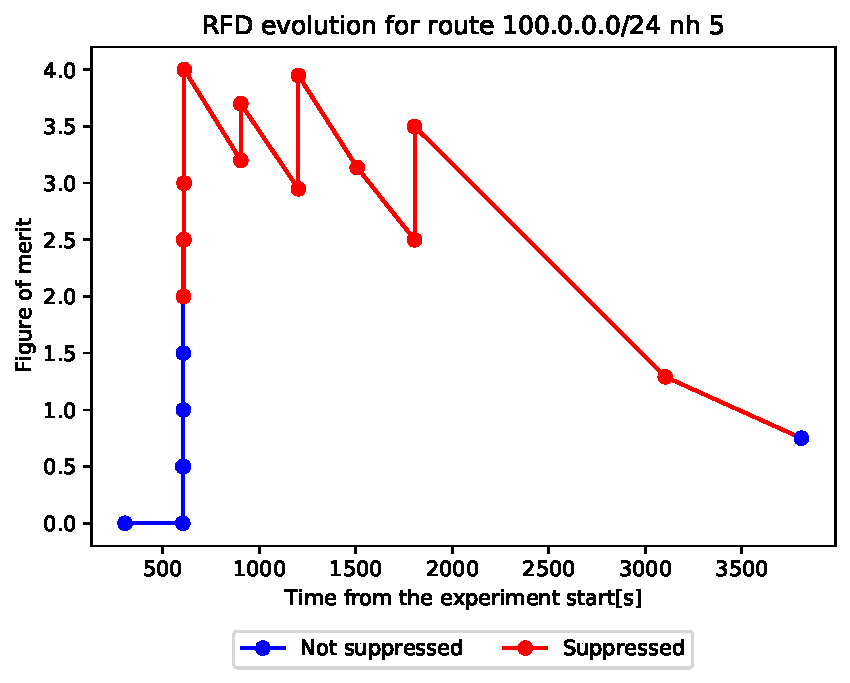
\includegraphics[width=\textwidth]{images/RFD/clique/FigureOfMerit/mrai1_RFD_x_rfd_R1.pdf}
         \caption{MRAI = 0s}
         \label{fig:clique_x_mrai0}
     \end{subfigure}
     \hfill
     \begin{subfigure}[b]{0.49\textwidth}
         \centering
         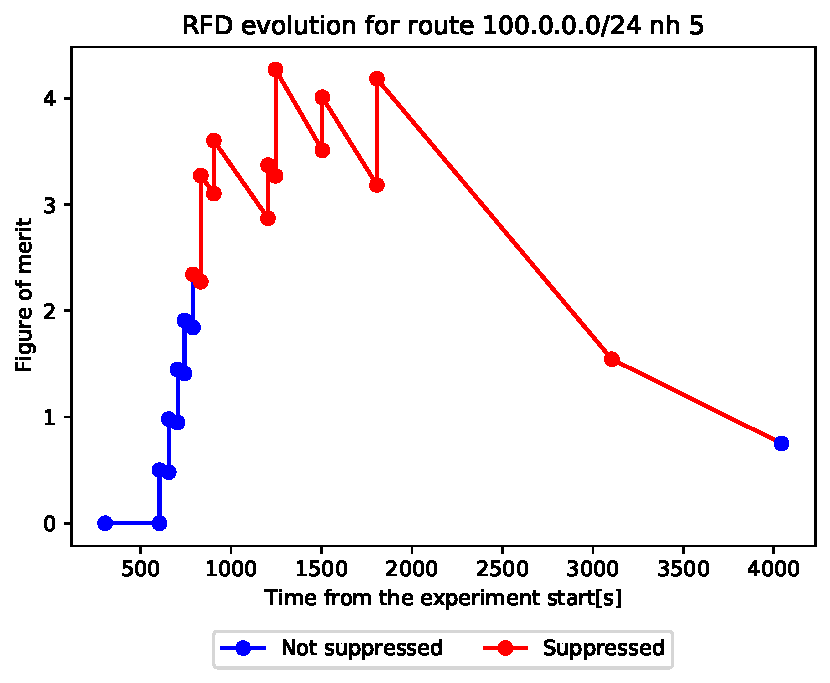
\includegraphics[width=\textwidth]{images/RFD/clique/FigureOfMerit/mrai11_RFD_x_rfd_R1.pdf}
         \caption{MRAI = 50s}
         \label{fig:clique_x_mrai50}
     \end{subfigure}
     \begin{subfigure}[b]{0.49\textwidth}
         \centering
         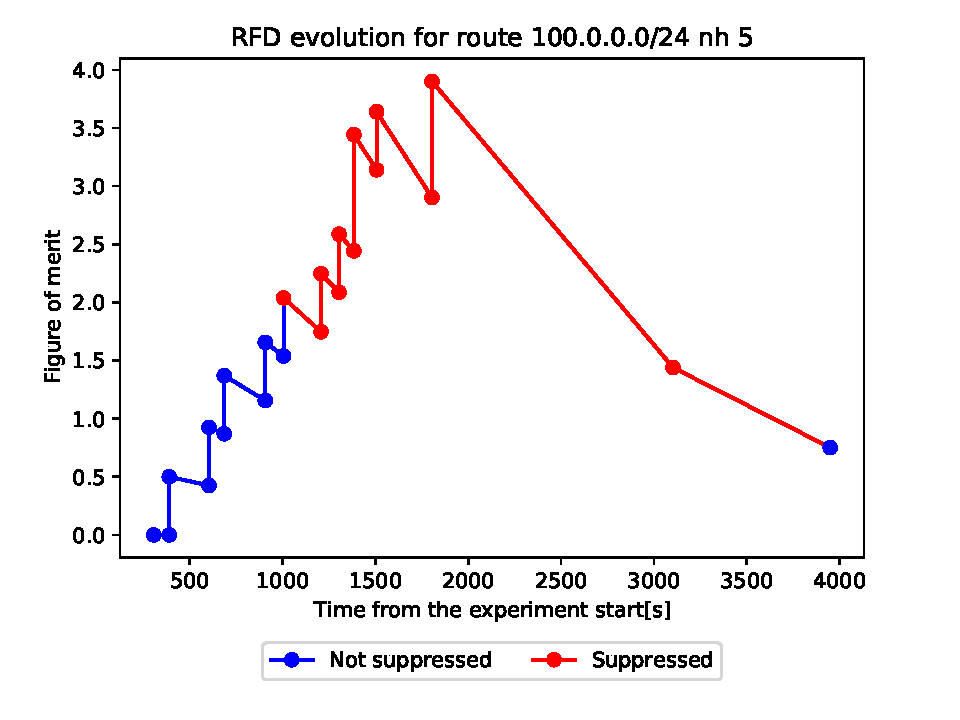
\includegraphics[width=\textwidth]{images/RFD/clique/FigureOfMerit/mrai21_RFD_x_rfd_R1.pdf}
         \caption{MRAI = 100s}
         \label{fig:clique_x_mrai100}
     \end{subfigure}
        \caption{Evolution of the figure of merit in the node X with different MRAIs,
		Clique graph, MRAI strategy fixed, signal "AWAWAWA", legacy RFD}
        \label{fig:clique_nodex}
\end{figure}

The node $x$ is a leaf of the network that will absorb everything the node \num{5}
sends to it.
In \Cref{fig:clique_nodex} is possible to see the evolution of the figure of merit
with different \ac{MRAI} values.
In the first case, with an \ac{MRAI} equal to \SI{0}{\second}, we will see a huge
spike caused by a lot of messages and route changes that the node \num{5} sends
to it.
While in the other two cases \Cref{fig:clique_x_mrai50,fig:clique_x_mrai100}
the \ac{MRAI} seems to not be much effective on the route through node \num{5}.
The messages are more delayed with high \ac{MRAI} but the growth of the figure
of merit has the same trend.
We can see that the route has been suppressed around \SI{1000}{\second}
and it is going to become available again around \SI{4000}{\second}.
In this period of time, from \SI{1000}{\second} to \SI{4000}{\second}, node $x$ still
receives some updates from node \num{5} that affects its best path, and this
makes the figure of merit evolve.
The evolution of the figure of merit stops around \SI{2000}{\second} that's because
also, the node \num{5} has suppressed the route, \Cref{fig:clique_node5}, and
doesn't send any more advertisements.
The point around \SI{3000}{\second} represent the moment when the route becomes
available again for node \num{5} that communicates the change to $x$.

\begin{figure}[h]
     \centering
     \begin{subfigure}[b]{0.49\textwidth}
         \centering
         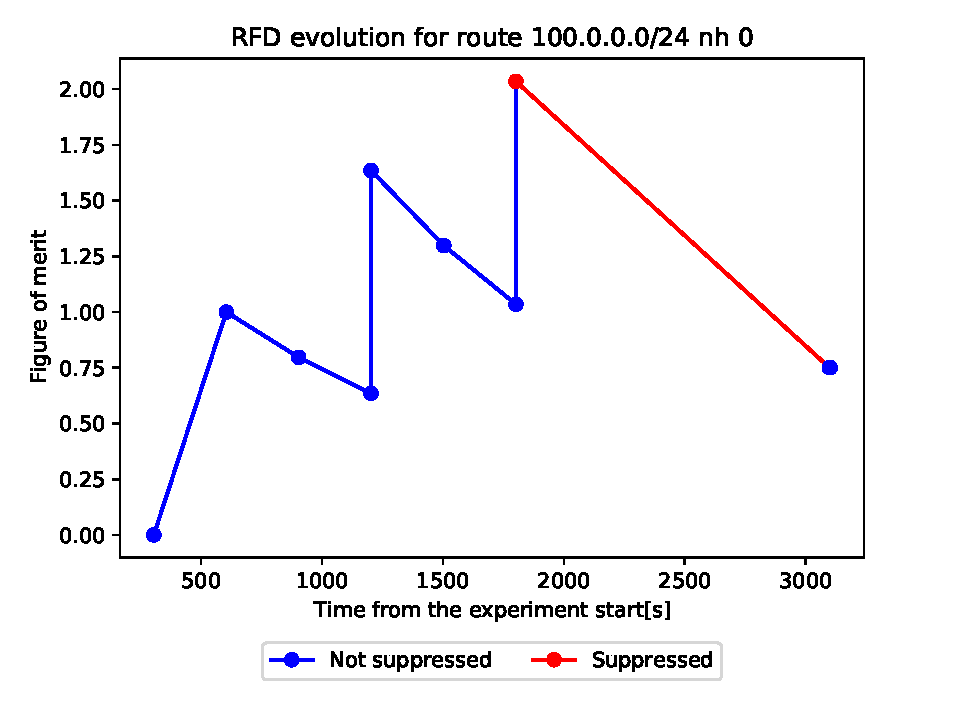
\includegraphics[width=\textwidth]{images/RFD/clique/FigureOfMerit/mrai1_RFD_5_rfd_R1.pdf}
         \caption{MRAI = 0s}
         \label{fig:clique_5_mrai0}
     \end{subfigure}
     \hfill
     \begin{subfigure}[b]{0.49\textwidth}
         \centering
         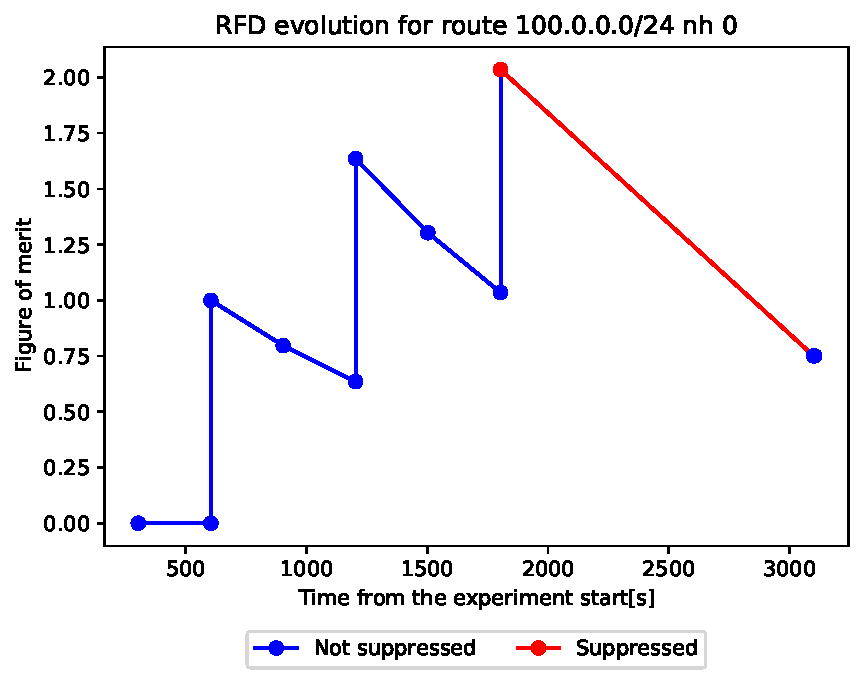
\includegraphics[width=\textwidth]{images/RFD/clique/FigureOfMerit/mrai11_RFD_5_rfd_R1.pdf}
         \caption{MRAI = 50s}
         \label{fig:clique_5_mrai50}
     \end{subfigure}
     \hfill
     \begin{subfigure}[b]{0.49\textwidth}
         \centering
         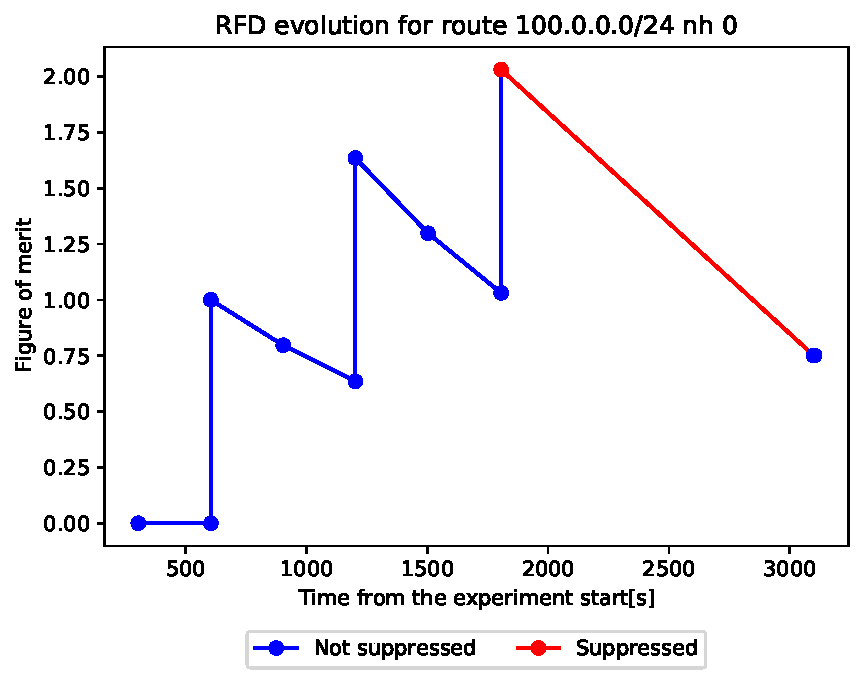
\includegraphics[width=\textwidth]{images/RFD/clique/FigureOfMerit/mrai21_RFD_5_rfd_R1.pdf}
         \caption{MRAI = 100s}
         \label{fig:clique_5_mrai100}
     \end{subfigure}
		\caption{Evolution of the figure of merit in the node \num{5} with different MRAIs.
		Clique graph, MRAI strategy fixed, signal "AWAWAWA", legacy RFD}
        \label{fig:clique_node5}
\end{figure}

The evolution of the figure of merit of the best path of node \num{5} is different
from the one of node $x$.
In fact, it is not influenced by \ac{MRAI} as we can see in \Cref{fig:clique_node5}.
That because the node \num{5} is directly connected to the node \num{0} that every
\SI{300}{\second} forward the message of $d$. \SI{300}{\second} are a delay large
enough to be not affected by the compression effect of \ac{MRAI}.
Around \SI{2000}{\second} node \num{5} suppress the route (as any other node in the
clique) and stops to forward it to node $x$ until \SI{3000}{\second} when it becomes
available again.

Node $x$ took almost \SI{4000}{\second} to converge because of the big fluctuations
of node \num{5} that suffers from the \textit{Path Exploration} problem, path
changes are considered bad behaviour in \ac{RFD}.

In conclusion, is not possible to notice an interaction between \ac{MRAI} and
\ac{RFD}, the differences are minor and the figure of merit growth is not
affected.
On the other hand, \ac{MRAI} can help to reduce the gap between the load that
the nodes have to handle.
If the number of messages is treatable, the convergence time given by the
environment that doesn't use \ac{RFD} is an overwhelming factor.

%\begin{itemize}
%    \item What is the impact of RFD?
%    \item In which occasion is present RFD?
%    \item Clique
%    \item Variations thanks to MRAI
%\end{itemize}

\section{RFC 7196 and MRAI}
\label{sec:bgp_rfd_comparison}

%The difference in the two \ac{RFC} that defines \ac{RFD} \cite{rfc2439,rfc7196}
%is in the parameters used.
%In fact, the \ac{RFC} \num{7196} modify the figure
%of merit threshold that is increased up to at least \num{6.0}, introducing
%two new set of possible \ac{RFD} filters that can be used:
%\begin{itemize}
%	\item \textit{\textbf{Aggressive}:} Suppression threshold no less than \num{6.0};
%	\item \textit{\textbf{Conservative}:} Suppression threshold no less than \num{12.0}.
%\end{itemize}
%
%Respectively \num{3} and \num{6} times the actual standard.
%
%I have then repeated the same experiments of \Cref{sec:bgp_rfd_toy} with the same
%clique graph, but with the two new \ac{RFD} strategies, the results are
%showed in \Cref{fig:clique_rfd7196}.

Like before I repeated the same experiments of \Cref{sec:rfd_2439_Vs_7196} with
different \ac{MRAI} settings.
In that section I was evaluating the two new techniques presented in~\cite{rfc7196},
which points to overcome some to restrictive settings of the original \ac{RFD}.
I have then evaluated the clique network with the \textit{Aggressive} and
\textit{Conservative} strategies and multiple \ac{MRAI} values.

The \ac{MRAI} \textit{Fixed} strategy has been used also in this experiments,
the set of possible values is \([0, 120]\) seconds.

The results are presented in \Cref{fig:clique_rfd7196}.

\begin{figure}[h]
     \centering
     \begin{subfigure}[b]{0.49\textwidth}
         \centering
         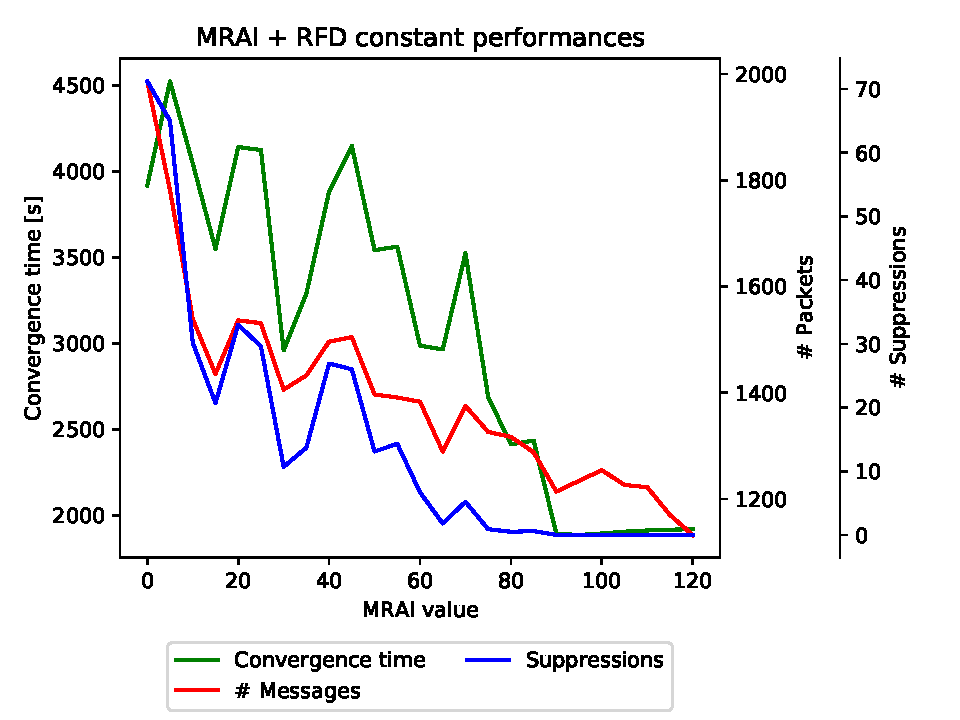
\includegraphics[width=\textwidth]{images/RFD/clique/cisco_clique10_RFD_7196_aggressive-constant_mrai_rfd_evolution.pdf}
         \caption{RFD 7196 Aggressive on the clique topology}
         \label{fig:rfd7196aggressive}
     \end{subfigure}
     \hfill
     \begin{subfigure}[b]{0.49\textwidth}
         \centering
         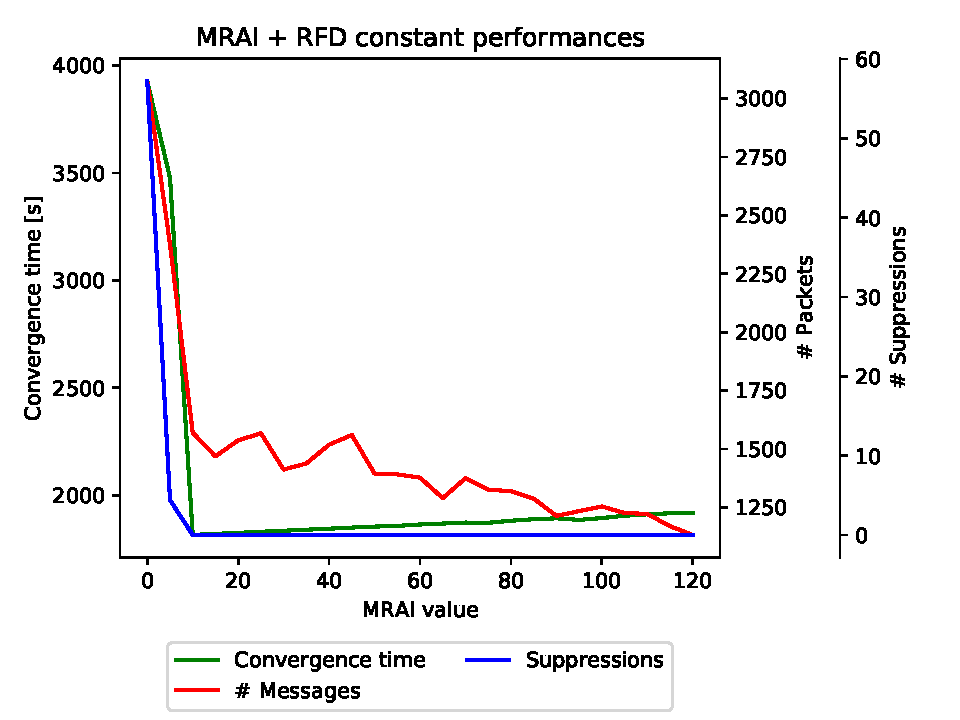
\includegraphics[width=\textwidth]{images/RFD/clique/cisco_clique10_RFD_7196_conservative-constant_mrai_rfd_evolution.pdf}
         \caption{RFD 7196 Conservative on the clique topology}
         \label{fig:rfd7196conservative}
     \end{subfigure}
		\caption{MRAI influence with different RFD strategies from \cite{rfc7196}.
		Clique graph, \ac{MRAI} \textit{Fixed}, signal \q{AWAWAWA}.}
        \label{fig:clique_rfd7196}
\end{figure}

We can see two completely different evolutions of the performances in \Cref{fig:clique_rfd7196}.
On the left plot, we can see the evolution with the \textit{Aggressive} strategy.
\ac{MRAI} is more effective to this strategy in respect to the standard one.
The number of suppressions fell down to almost \num{0} with an \ac{MRAI} near
\SI{90}{\second}.
The message trend is similar to the one of the case without \ac{RFD} but with an
important difference in the case of  \ac{MRAI} equal \SI{0}{\second}, the number
of average messages is around \num{2600} in respect of the \num{10000} without
\ac{RFD}.
While with a high \ac{MRAI} the message trends are similar and equal when the number of
suppressions reach \num{0}.

The convergence time, on the other hand, has a different trend in respect of
the one that we saw in \Cref{fig:clique_evolution_rfd}.
It is stable until \ac{MRAI} reaches \SI{70}{\second}, at that point, the number
of message reduction permits to avoid multiple suppressions.
This gain in the suppressions has a positive effect on the convergence time that
fell down.
When \ac{MRAI} permits to have \num{0} suppression the convergence time trend
starts to act as the \textit{NoRFD} case.
While, before \ac{MRAI} equal \SI{60}{\second}, the number of suppression is half
in respect of the standard case but the convergence time is not affected.

In \Cref{fig:rfd7196conservative} we can see the evolution of the network with the
\textit{Conservative} strategy, the threshold of this strategy is the double of
the \textit{Aggressive} one.
The effects of this difference are huge, is sufficient an \ac{MRAI} of \SI{10}{\second}
to avoid at all any suppression, causing the trends, in terms of messages and
convergence time, to be equal to the \textit{No\ac{RFD}} case.
Also with an \ac{MRAI} of \SI{0}{\second} is possible to see a difference in
terms of messages and convergence time in respect of the other two strategies.
This is the strategy that more likely resembles the \textit{NoRFD} one,
having a convergence time incredibly more low, at the cost of few hundreds of messages.

We can now take a look more closely to what happens to the figure of merit
for the only route that node $x$ receives with an \ac{MRAI} of \SI{30}{\second}.
Results are showed in \Cref{fig:clique_nodex_rfd7196Aggressive}, reporting
the evolution of the figure of merit in the \textit{Aggressive} strategy.
The \textit{Conservative} case is not presented because it is never going to suppress
the route.

\begin{figure}[h]
     \centering
     \begin{subfigure}[b]{0.49\textwidth}
         \centering
         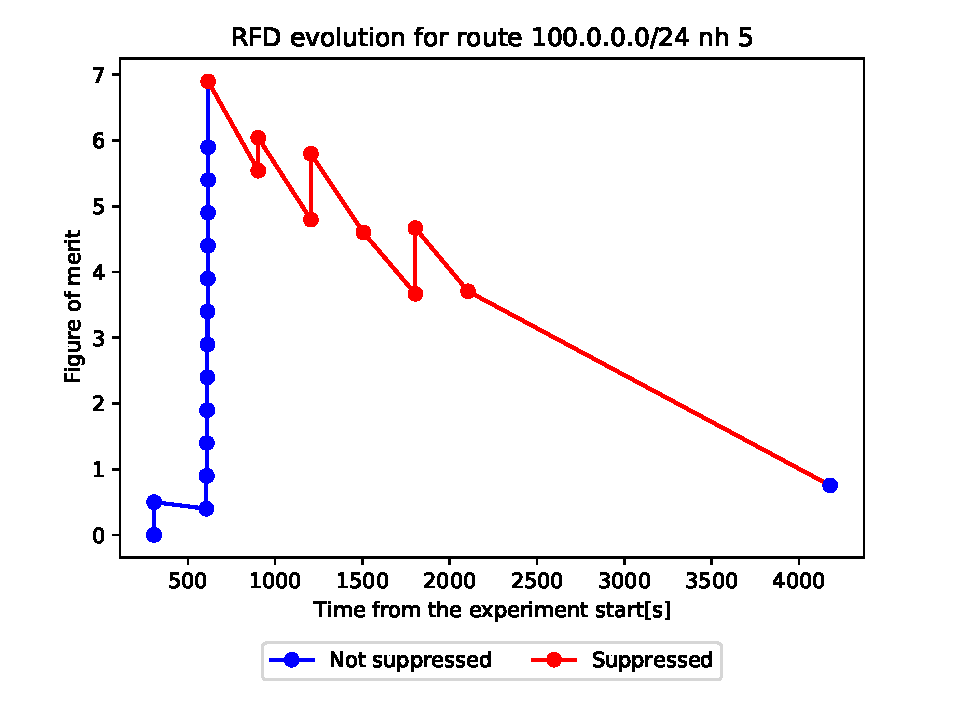
\includegraphics[width=\textwidth]{images/RFD/clique/FigureOfMerit/mrai1_RFD_7196_aggressive_x_rfd_R1.pdf}
         \caption{MRAI = 0s, RFD 7196 Aggressive}
         \label{fig:clique_x_mrai0_rfd7196Aggressive}
     \end{subfigure}
     \hfill
     \begin{subfigure}[b]{0.49\textwidth}
         \centering
         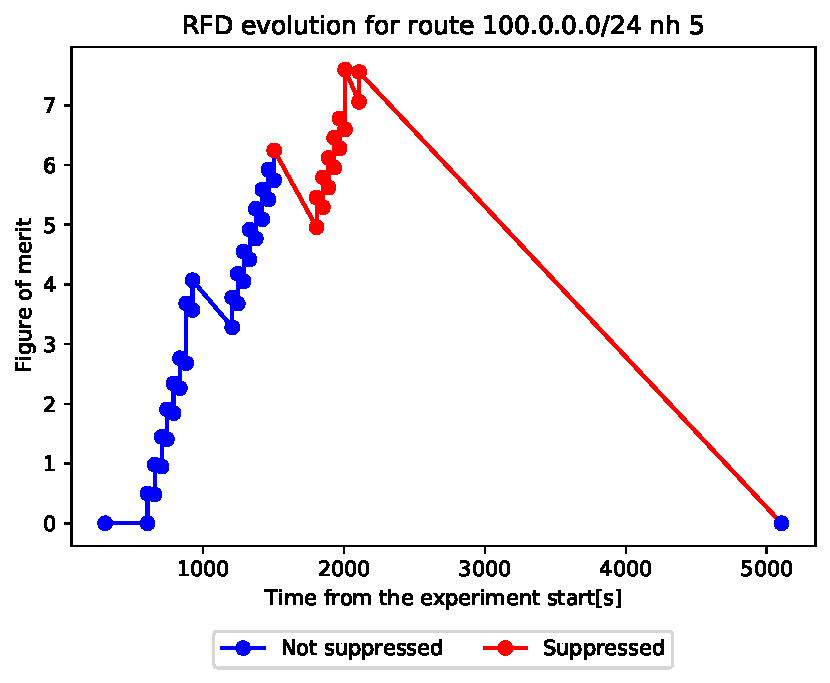
\includegraphics[width=\textwidth]{images/RFD/clique/FigureOfMerit/mrai11_RFD_7196_aggressive_x_rfd_R1.pdf}
         \caption{MRAI = 50s, RFD 7196 Aggressive}
         \label{fig:clique_x_mrai50_rfd7196Aggressive}
     \end{subfigure}
     \begin{subfigure}[b]{0.49\textwidth}
         \centering
         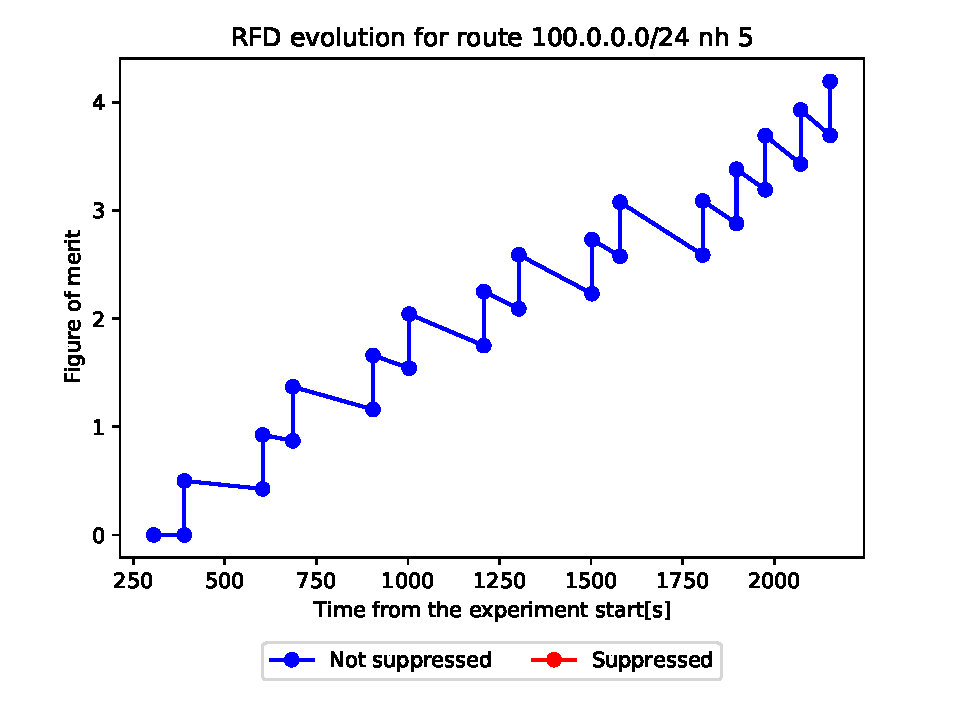
\includegraphics[width=\textwidth]{images/RFD/clique/FigureOfMerit/mrai21_RFD_7196_aggressive_x_rfd_R1.pdf}
         \caption{MRAI = 100s, RFD 7196 Aggressive}
         \label{fig:clique_x_mrai100_rfd7196Aggressive}
     \end{subfigure}
        \caption{Evolution of the figure of merit in the node X with different
				MRAIs, with RFD 7196 aggressive in a clique topology}
        \label{fig:clique_nodex_rfd7196Aggressive}
\end{figure}

We can see in \Cref{fig:clique_x_mrai0_rfd7196Aggressive,fig:clique_x_mrai50_rfd7196Aggressive}
that \ac{MRAI} plays an important role in the figure of merit of node $x$.
In the first case, the route would be delayed up to \SI{4000}{\second} with a
suppression value that touches \num{12} few seconds after the first flap.
In the second one, the growth is slower but it passes the threshold around
\SI{1800}{\second} reaching a value of \num{7}.
For this reason, it requires a higher time to become available again.
We can also notice that the route become available with a figure of merit of
\num{0}, that's because it has been triggered the max suppression threshold,
with the default value of cisco after \SI{1}{\hour} a route would become available
again, no matter the evolution of the figure of merit.
With a higher \ac{MRAI} node \num{5} is able to compress more routes, the effects
are visible in \Cref{fig:clique_x_mrai100_rfd7196Aggressive}, where the figure of
merit never goes over the threshold.

In conclusion, if \ac{MRAI}, with the standard \ac{RFD}, was playing a more
marginal role because of the restrictive threshold, now, with those strategies,
it plays a more relevant position and acts as a key factor between the suppression
or not of a route.
Also, is possible to notice that the simple increment of the threshold should be
accompanied by a reconfiguration of the other parameters, otherwise the overpassing
of the threshold would require a longer time to reactivate the route.

%\begin{itemize}
%    \item Time comparison between both of them
%    \item how them react differently?
%    \item why?
%\end{itemize}

%\section{Mice VS Elephants}
%\label{sec:bgp_rfd_mice_vs_elephants}

%From the work of R. Bush et al., \cite{pelsser2011route} we know that the majority
%of the \ac{ADV} that are transmitted on the Internet are from a small set of \acp{AS}.
%Those \acp{AS} with their flaps causes update storms almost continuously.
%I report a figure form \cite{pelsser2011route} for simplicity in
%\Cref{fig:RBushPrefixes}
%Thanks to the studies of
%\ac{APNIC}\footnote{\href{https://blog.apnic.net/2020/01/15/bgp-in-2019-bgp-churn/}{APNIC BGP 2019 report}}
%we also know that this behaviour is still present nowadays, the \Cref{fig:apnicPrefixes}
%is taken from one of their annual reports and shows that \num{10}\% of
%all the active prefixes produce more or less the \num{70}\% of the total
%messages received.
%
%\begin{figure}[h]
%     \centering
%     \begin{subfigure}[b]{0.48\textwidth}
%         \centering
%         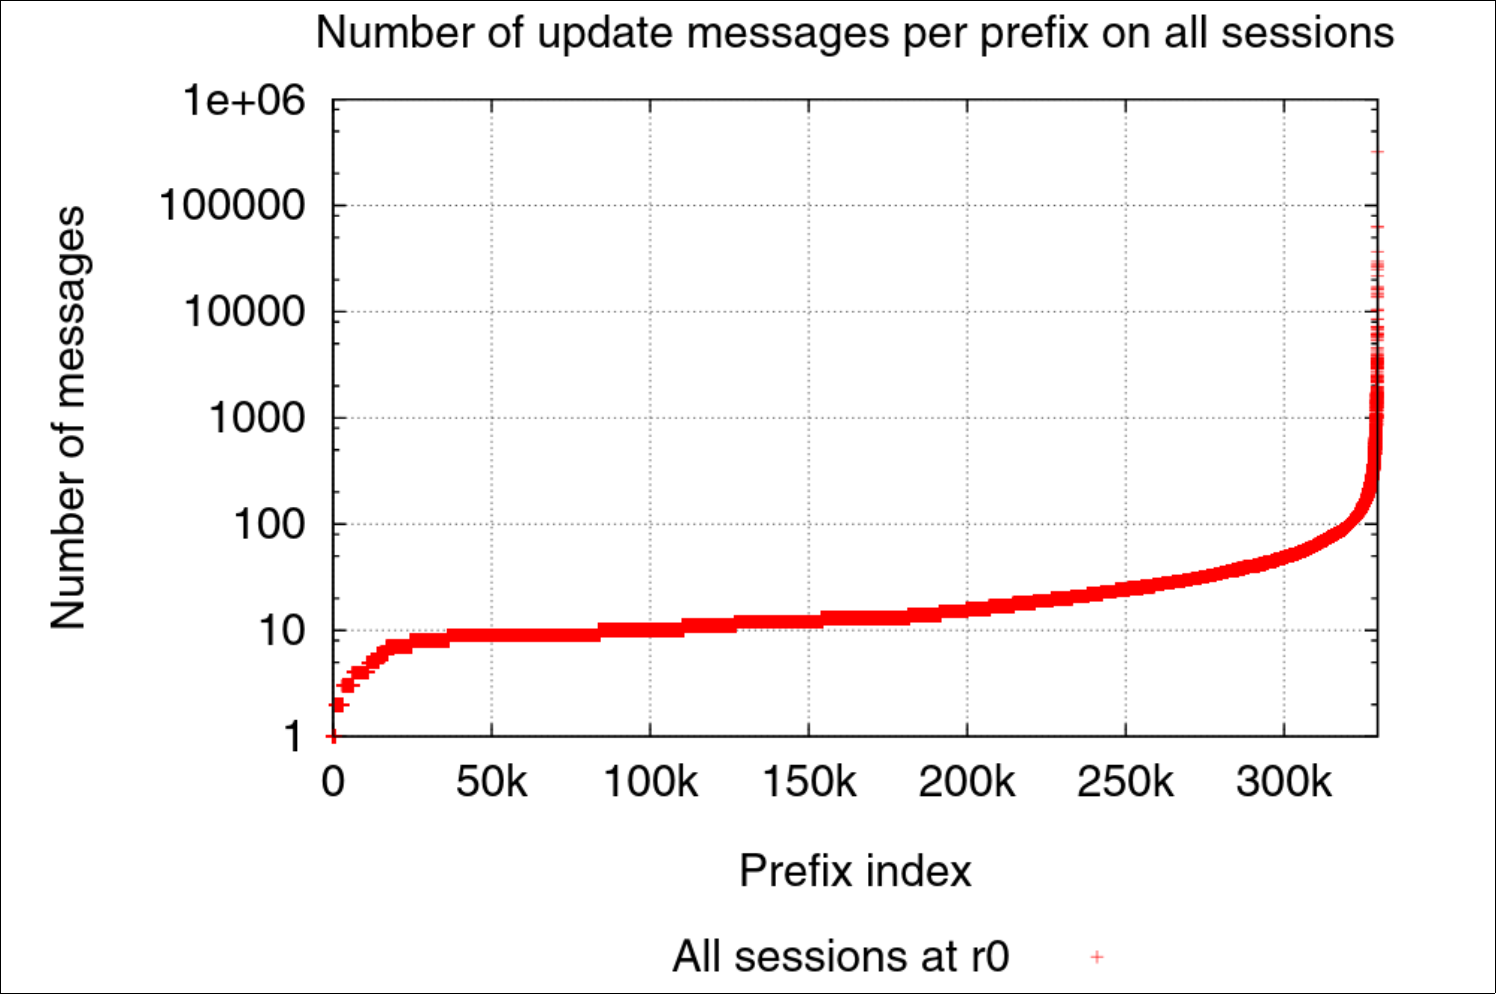
\includegraphics[width=\textwidth]{images/RFD/miceVSelephants/prefixVSmessagesRbush.png}
%		 \caption{Prefixes and number of updates associated, figure from \cite{pelsser2011route}}
%         \label{fig:RBushPrefixes}
%     \end{subfigure}
%     \hfill
%     \begin{subfigure}[b]{0.48\textwidth}
%         \centering
%         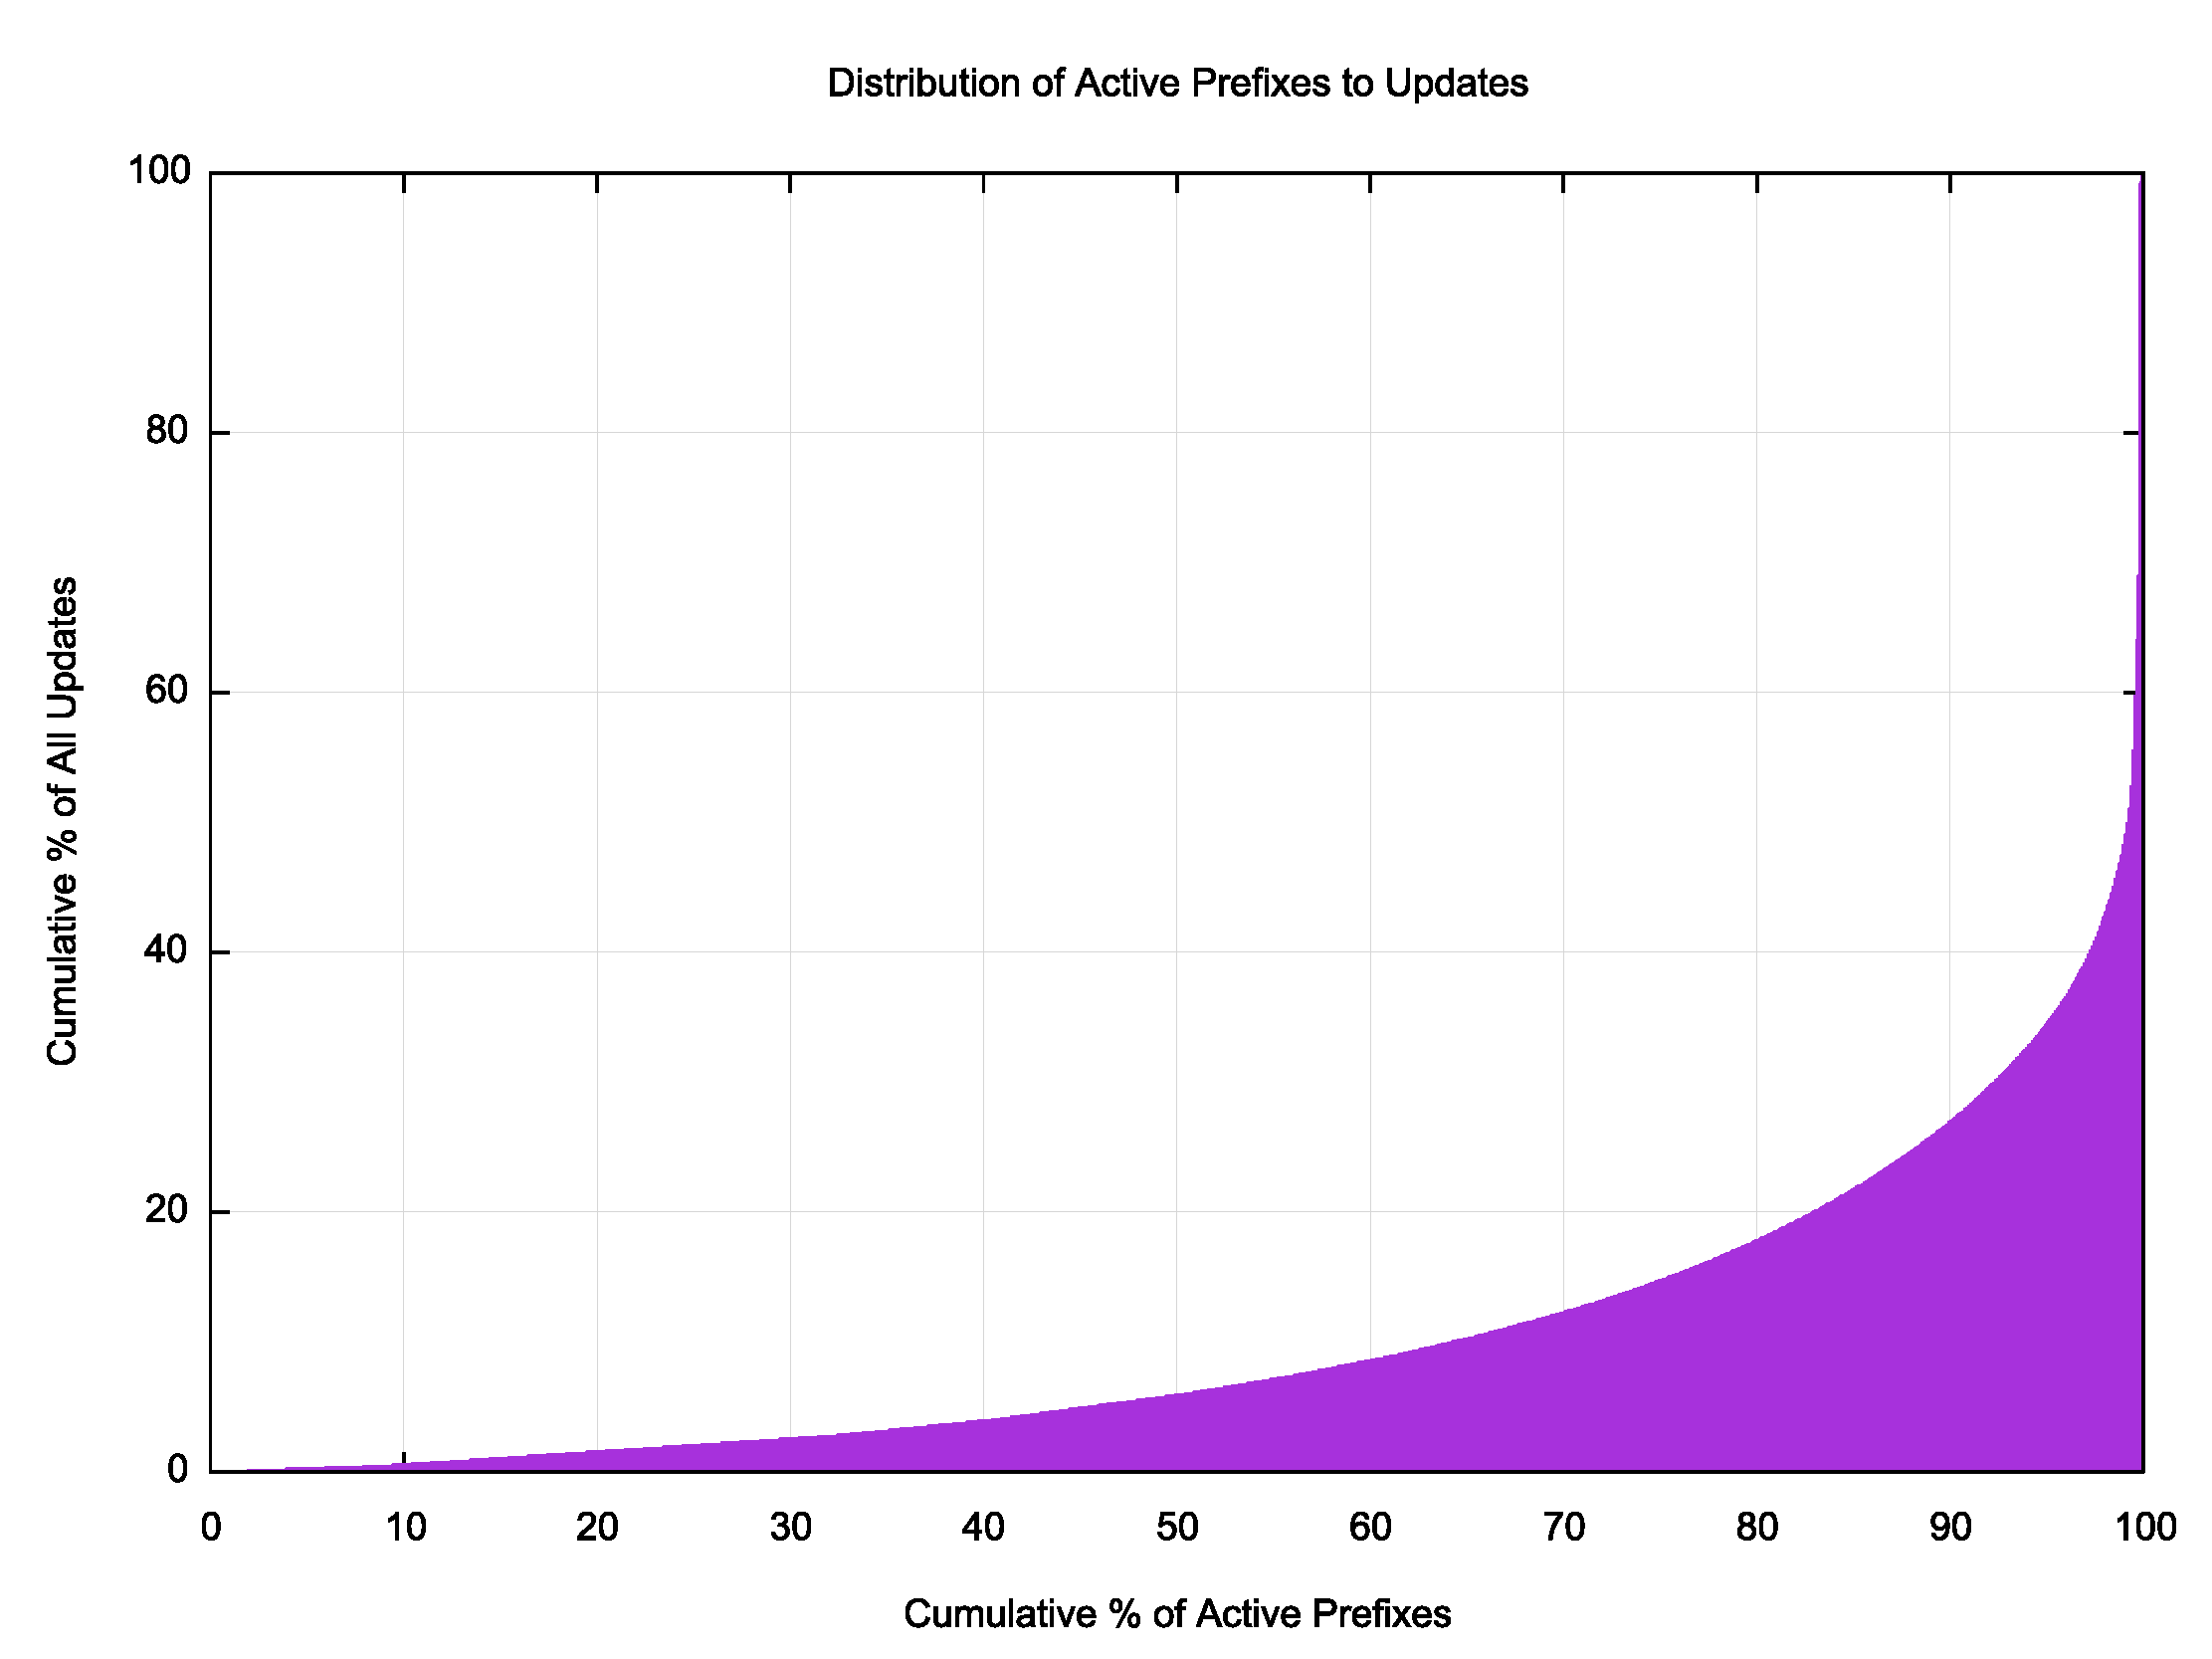
\includegraphics[width=\textwidth]{images/RFD/miceVSelephants/bgp2fig5-pfx-upds-cuml.png}
%         \caption{Prefixes and number of updates associated, [apnic 2019]}
%         \label{fig:apnicPrefixes}
%     \end{subfigure}
%        \caption{Prefixes influence on updates}
%        \label{fig:prefixVSmessages}
%\end{figure}
%
%We can then divide those prefixes in two sets:
%\begin{itemize}
%	\item \textbf{\textit{Mice}}, this set represent the majority of the prefixes,
%		all the prefixes that does not generate more than \num{100} updates
%		in \Cref{fig:RBushPrefixes}
%	\item \textbf{\textit{Elephants}}, this set represent the remaining part
%		of the prefixes, those that produces the majority of the messages.
%\end{itemize}
%
%Thanks to a annual review of \ac{BGP} by APNIC, presented at RIPE 52 \cite{huston2006bgp},
%we can also have an example of those elephants prefixes.
%This example is shown in \Cref{fig:ripePrefixFlaps}, it takes in consideration the
%prefix \q{202.64.49.0/24} showing that in a relatively small period of time it has
%produced thousands of \ac{ADV} per day.
%In this case, this particular prefix has produced \num{198,370} \ac{ADV} producing
%in total \num{96,330} flaps.
%
%\begin{figure}[h]
%    \centering
%    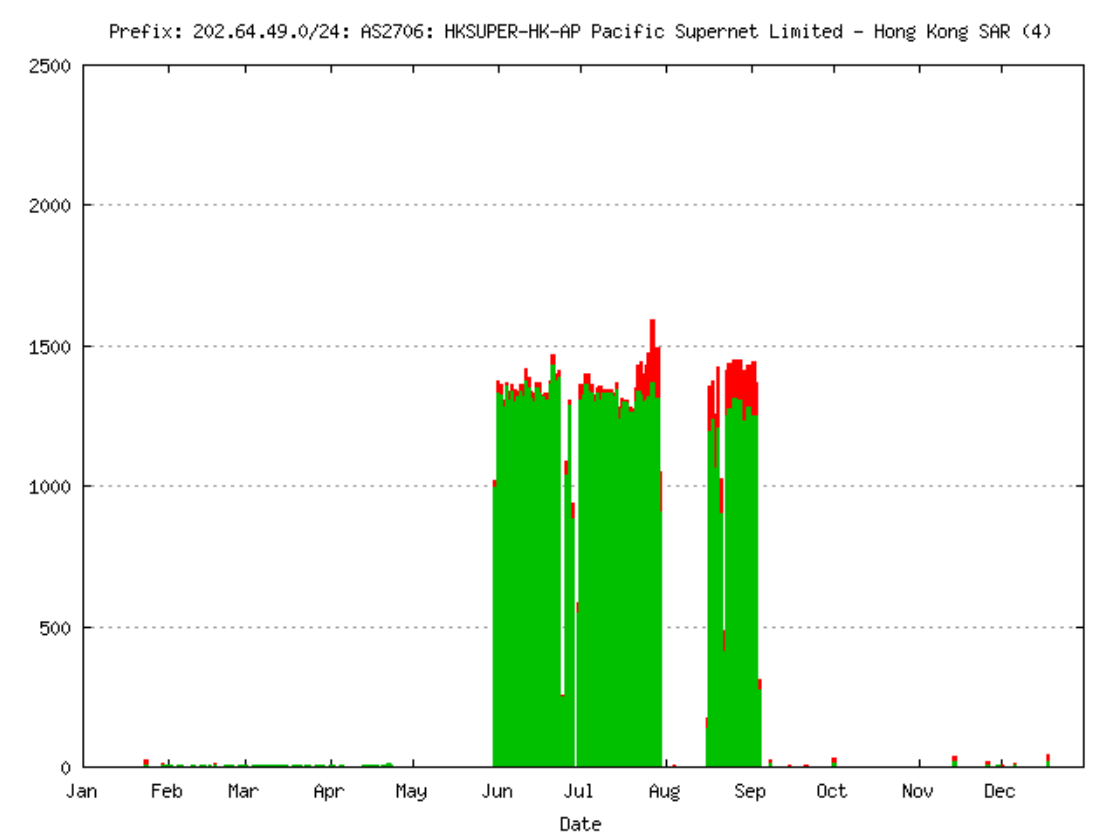
\includegraphics[scale=0.22]{images/RFD/miceVSelephants/ripePrefixFlap.png}
%	\caption{202.64.49.0/24 flaps plot from \cite{huston2006bgp}}
%    \label{fig:ripePrefixFlaps}
%\end{figure}
%
%I have then used this data to configure two new environments for the simulations.
%The first one points to reproduce the \textit{Mice} behaviour, the second
%one the \textit{Elephants}.
%
%In both these environments, I have then compared the four different strategies of
%\ac{RFD}, \textit{NoRFD}, standard \ac{RFD} from the \ac{RFC} \num{2439}
%and the two from \cite{rfc7196}.
%
%The topology used for those experiments is an \textit{Internet like} topology
%with \num{1000} nodes and \ac{MRAI} is fixed to \SI{30}{\second} for all the links.
%The source of the signal has been chosen randomly on the graph.
%For each experiment has been executed \num{50} runs.

%\subsection{Mice}
%\label{subsec:mice}

%The particularity of the \textit{Mice} experiments is in the signal, we have
%a low number of flaps interleaved by a long timer.
%I have then used a signal with \num{5} flaps, \q{AWAWAWAWAWA} with a delay
%of \SI{300}{\second} (\SI{5}{\minute}) between each message.
%The results are presented in \Cref{fig:1000_RFD_MRAI30_mice_bis}.
%I have executed \num{50} runs for each \ac{RFD} strategy.
%
%\begin{figure}[h]
%     \centering
%     \begin{subfigure}[b]{0.325\textwidth}
%         \centering
%         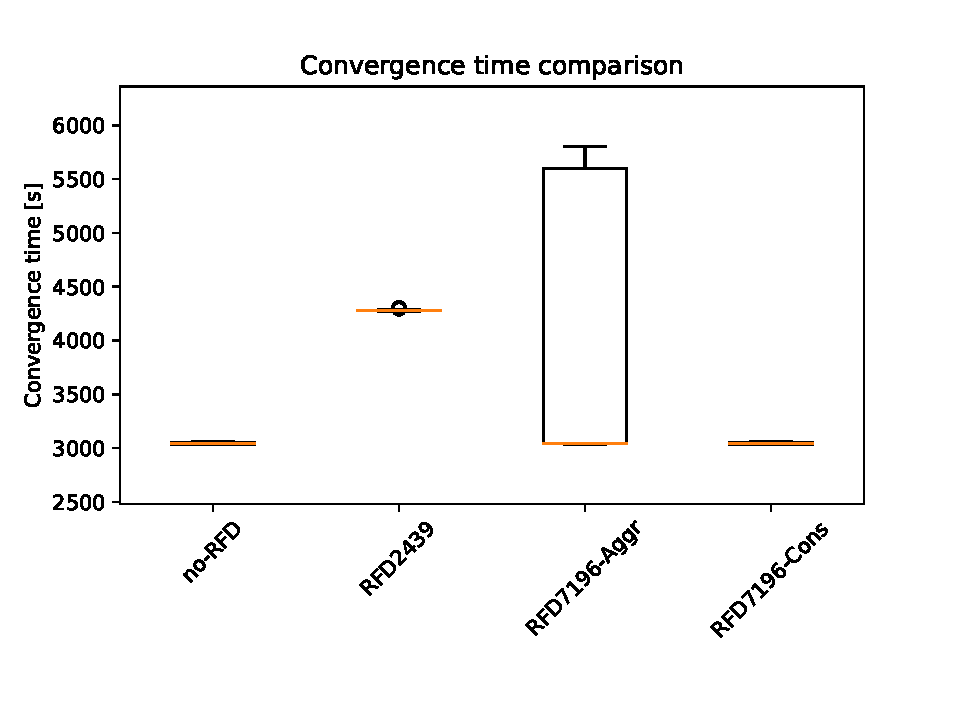
\includegraphics[width=\textwidth]{images/RFD/miceVSelephants/mice/cisco_1000MRAI30_rfd_comparison_time_boxplot.pdf}
%         \caption{Convergence time respect to the RFD strategy}
%         \label{fig:1000_RFD_MRAI30_mice_time_bis}
%     \end{subfigure}
%     \hfill
%     \begin{subfigure}[b]{0.325\textwidth}
%         \centering
%         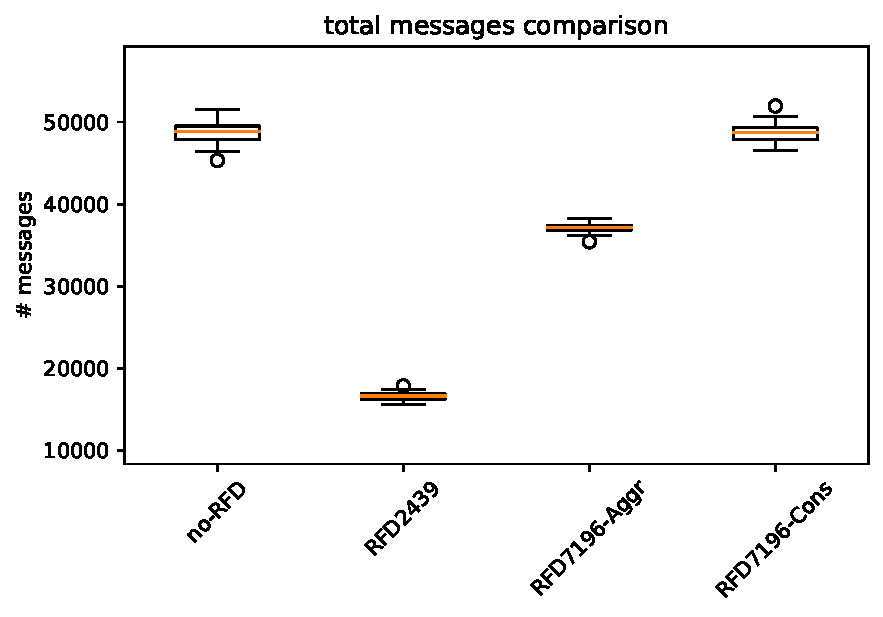
\includegraphics[width=\textwidth]{images/RFD/miceVSelephants/mice/cisco_1000MRAI30_rfd_comparison_messages_boxplot.pdf}
%         \caption{Number of messages respect to the RFD strategy}
%         \label{fig:1000_RFD_MRAI30_mice_messages_bis}
%     \end{subfigure}
%     \hfill
%     \begin{subfigure}[b]{0.325\textwidth}
%         \centering
%         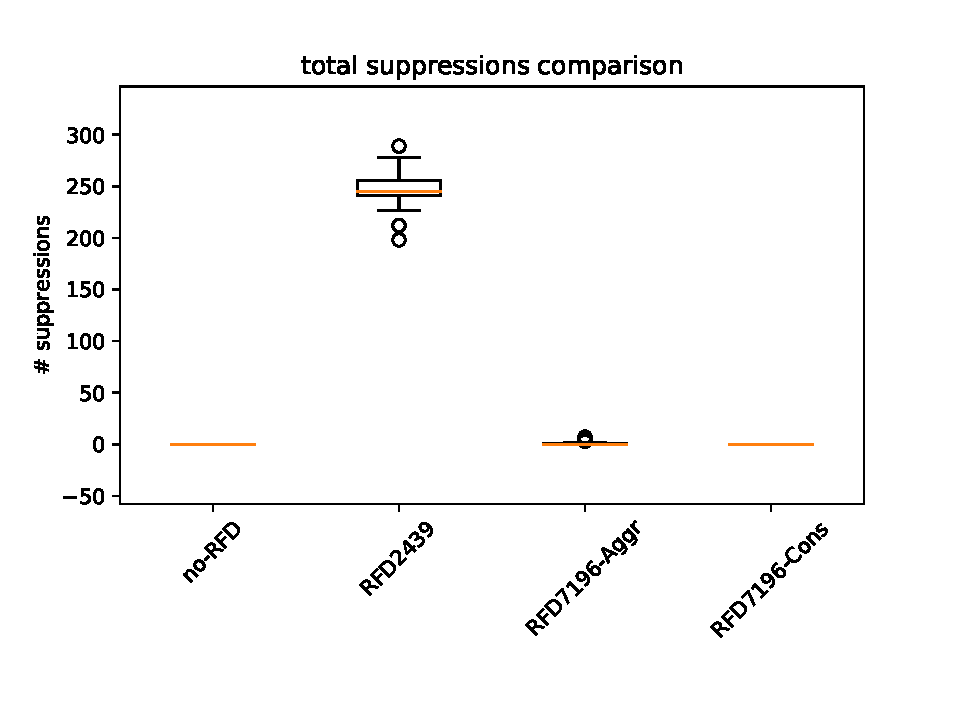
\includegraphics[width=\textwidth]{images/RFD/miceVSelephants/mice/cisco_1000MRAI30_rfd_comparison_suppressions_boxplot.pdf}
%         \caption{Number of suppressions respect to the RFD strategy}
%         \label{fig:1000_RFD_MRAI30_mice_suppressions_bis}
%     \end{subfigure}
%		\caption{Internet like topology 1000 nodes, MRAI=30s, random destination,
%		5 flaps, \SI{300}{\second} message delay, Network performances,
%		\num{50} runs per strategy.}
%        \label{fig:1000_RFD_MRAI30_mice_bis}
%\end{figure}
%
%From \Cref{fig:1000_RFD_MRAI30_mice_suppressions_bis} we can see that there is a
%big difference in the number of suppression.
%The standard strategy produces on average almost \num{1500} suppressions and the effects
%of those suppressions can be seen in \Cref{fig:1000_RFD_MRAI30_mice_time_bis,fig:1000_RFD_MRAI30_mice_messages_bis}.
%On average, it presents a convergence time higher than \SI{6000}{\second}
%but with a number of total messages transmitted around \num{16000} with a very
%low variance.
%A different case is presented by the \textit{Conservative} strategy from \ac{RFC}
%7196 \cite{rfc7196}.
%The threshold in this last case is so permissive that we have a really small
%number of suppression.
%For this reason, the number of messages transmitted, on average, is similar to
%the \textit{NoRFD} case, around \num{50000}.
%While, the convergence time is around \SI{6500}{\second}, like the standard \ac{RFD}
%strategy.
%This proves that few suppression can heavily influence the network performances,
%in particular the convergence time.
%Also because the recover from a suppression with a higher threshold would require
%more time.
%
%In the middle we find the \textit{Aggressive} strategy, we can see from the
%suppression boxplot that it produces a smaller number of suppression in respect
%of the legacy strategy with a smaller variance.
%Also, the convergence time respect this trend, in fact, the average time is
%below \SI{6000}{\second}.
%While The number of messages transmitted is more than double in respect
%of the strategy described by the \ac{RFC} \num{2439}.
%
%We can then conclude that a small number of suppression can affect both the
%performances, like the few suppressions in the \textit{Conservative} strategy
%for the convergence time.
%Also, the few missing suppression in the \textit{Aggressive} strategy will
%enormously impact the number of messages transmitted.
%
%Is also possible to study which are the nodes that produce the suppression and how
%far are them from the signal source.
%We can see the results of this study, for each suppression technique in \Cref{fig:1000_RFD_centVSsup}.
%
%\begin{figure}[h]
%     \centering
%     \begin{subfigure}[b]{0.325\textwidth}
%         \centering
%         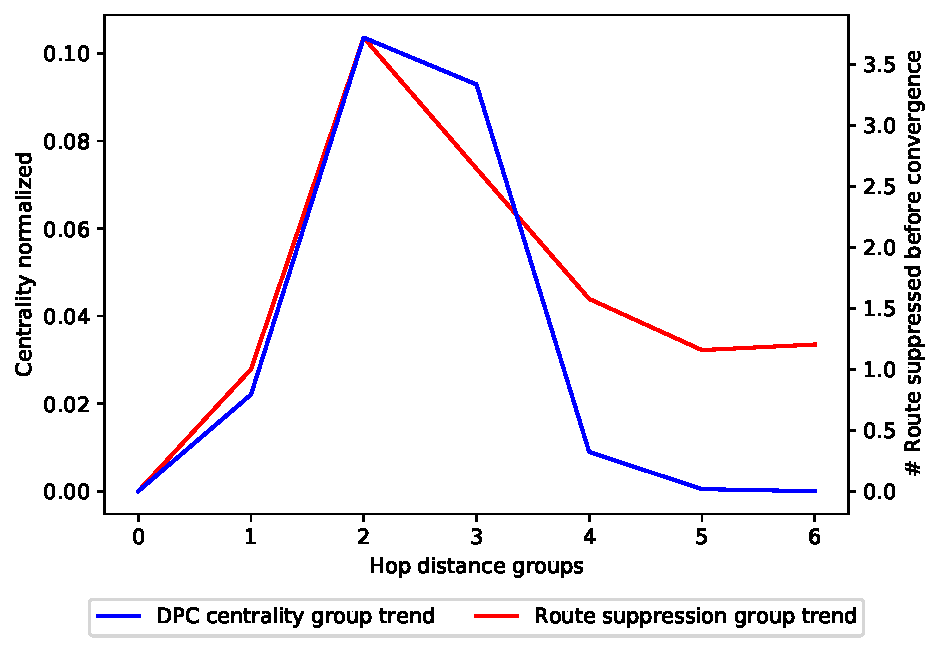
\includegraphics[width=\textwidth]{images/RFD/miceVSelephants/mice/cisco_1000_RFD_nodeConvergence_centVSsup_trend.pdf}
%         \caption{RFD 2439 Strategy}
%         \label{fig:1000_2439RFD_centVSsup}
%     \end{subfigure}
%     \hfill
%     \begin{subfigure}[b]{0.325\textwidth}
%         \centering
%         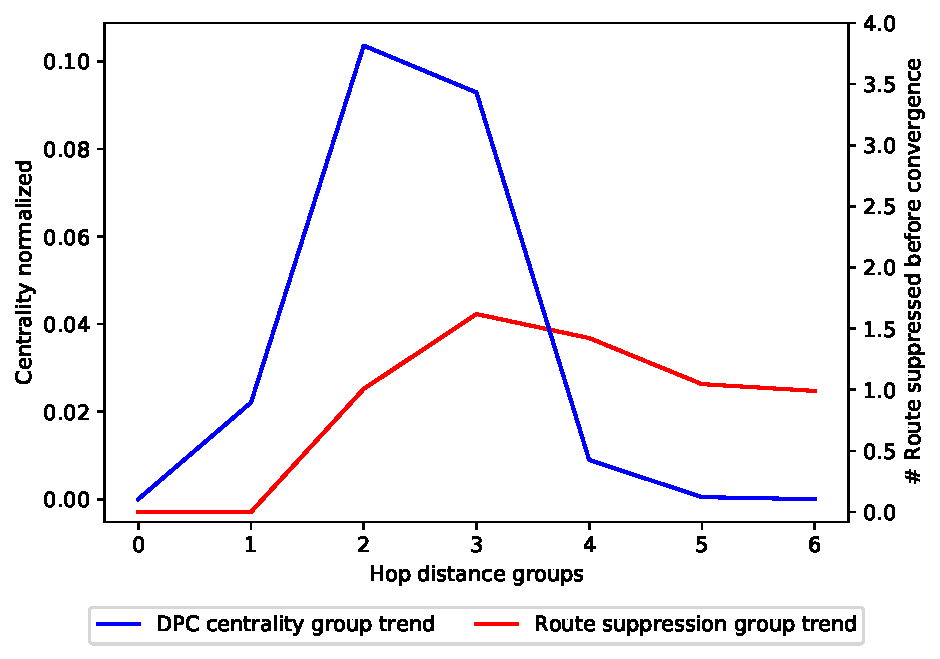
\includegraphics[width=\textwidth]{images/RFD/miceVSelephants/mice/cisco_1000_RFD_7196_aggressive_nodeConvergence_centVSsup_trend.pdf}
%         \caption{RFD 7196 Aggressive Strategy}
%         \label{fig:1000_7196RFDA_centVSsup}
%     \end{subfigure}
%     \hfill
%     \begin{subfigure}[b]{0.325\textwidth}
%         \centering
%         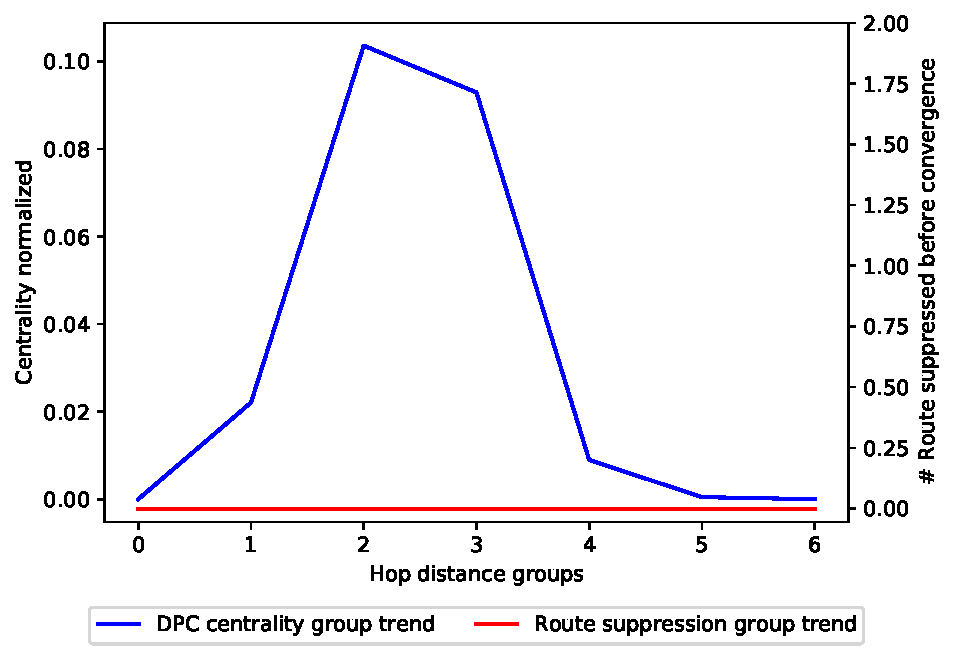
\includegraphics[width=\textwidth]{images/RFD/miceVSelephants/mice/cisco_1000_RFD_7196_conservative_nodeConvergence_centVSsup_trend.pdf}
%         \caption{RFD 7196 Conservative Strategy}
%         \label{fig:1000_7196RFDC_centVSsup}
%     \end{subfigure}
%		\caption{Internet like topology \num{1000} nodes, \ac{MRAI} = \SI{30}{\second}, random destination, \num{5} flaps, \SI{300}{\second} between messages, Suppression trend VS avg hop centrality}
%        \label{fig:1000_RFD_centVSsup}
%\end{figure}
%
%For the plots in \Cref{fig:1000_RFD_centVSsup} the $x$ axis represent the distance
%from the source node in terms of hops and all the other nodes are grouped by this
%distance.
%The blue line represents the average centrality of the groups, for each node of the
%graph I calculated the centrality using the \ac{DPC} metric then grouped them
%and calculated the average value.
%As expected the central nodes have a higher centrality and them are a few hops
%of distance
%from the source node.
%The centrality trend is equal for each plot in \Cref{fig:1000_RFD_centVSsup}
%because the graph and the source node are the same for each experiment.
%
%The red line represents the average number of suppressions per group.
%As we can see with the standard strategy, \Cref{fig:1000_2439RFD_centVSsup},
%on average, the route has been blocked \num{1} time by the nearest nodes and then,
%this value increase reaching the center clique up to \num{3.5} times and then
%slowly decreases in the following groups.
%In the farthest group, we will still see on average \num{1} suppression.
%The \textit{Aggressive} strategy, \Cref{fig:1000_7196RFDA_centVSsup} present
%a similar behaviour, the nearest nodes don't block the route, while the central
%nodes start blocking it with a maximum average of \num{1.6} times.
%After those central nodes, the farthest nodes, that have a low centrality will
%block it on average \num{1} time, like the legacy strategy.
%The \textit{Conservative} strategy, presented in \Cref{fig:1000_7196RFDC_centVSsup},
%has a different trend.
%We can see that the central nodes do not block the route, while only the farthest
%ones block it a few times, with an average value of \num{0.2} times.
%This can give us some hints, a very high threshold can promote the path
%exploration problem that will cause multiple update storms in farthest nodes.
%
%From those experiments we can see that having a higher threshold could help
%to spread the knowledge near the source of the flaps, but once the
%\textit{Path exploration} problem takes over, the nodes are going to suppress
%the destination.
%This is a good behaviour because it circumscribes an area in which the
%information can spread instead of blocking it almost everywhere.
%Those few suppression can highly impact in general the average convergence rate
%of the network.
%Is important to consider that a higher threshold means also a higher time to
%make the destination available again, maybe a new decay function should be considered.

%\subsection{Elephants}
%\label{subsec:bgp_elephants}

%The elephants prefixes, as I mentioned in \Cref{sec:bgp_rfd_mice_vs_elephants},
%are the ones that produce the majority of the \ac{ADV}.
%And we also know, thanks to \cite{huston2006bgp}, that is possible to see over
%thousands of messages per day.
%For this reason, the \textit{elephants} environment signal is composed of \num{100}
%flaps, with a delay between the messages of \SI{3}{\second}.
%All the other properties of the environment are unchanged.
%The results are presented in \Cref{fig:1000_RFD_MRAI_30_elephant,fig:1000_RFD_cent_VS_sup_elephants}.
%
%\begin{figure}[h]
%     \centering
%     \begin{subfigure}[b]{0.325\textwidth}
%         \centering
%         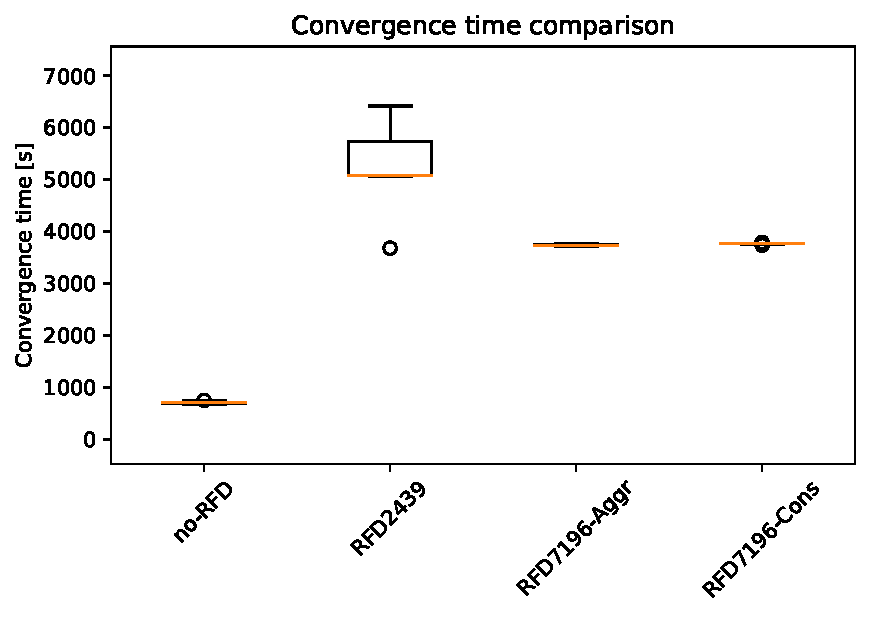
\includegraphics[width=\textwidth]{images/RFD/miceVSelephants/elephants/cisco_1000MRAI30_rfd_comparison_time_boxplot.pdf}
%         \caption{Convergence time respect to the RFD strategy}
%         \label{fig:1000_RFD_MRAI_30_time_elephant}
%     \end{subfigure}
%     \hfill
%     \begin{subfigure}[b]{0.325\textwidth}
%         \centering
%         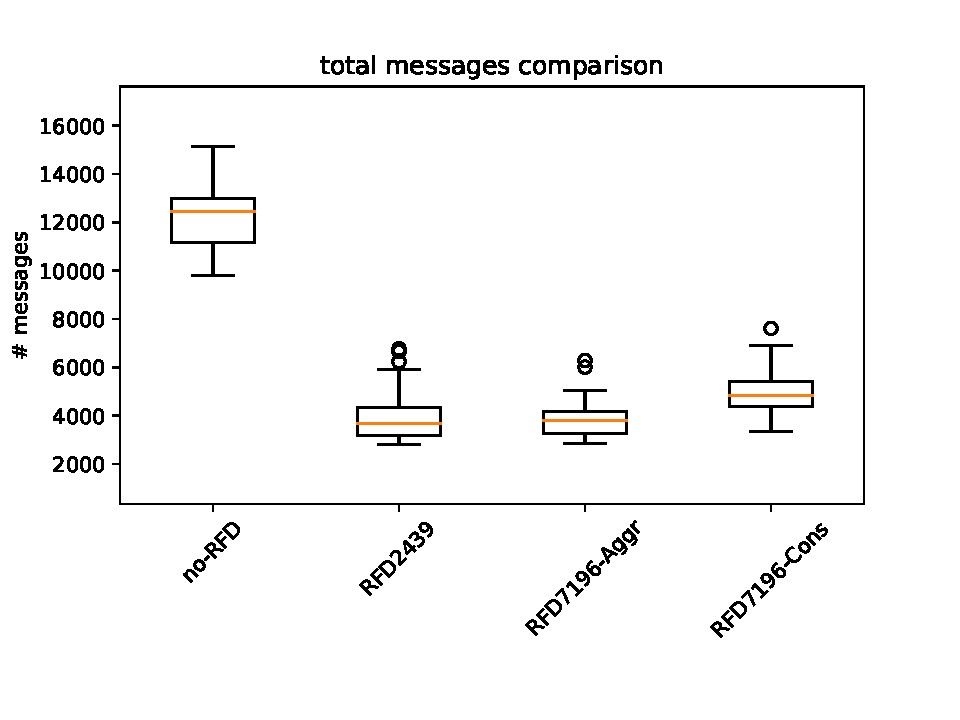
\includegraphics[width=\textwidth]{images/RFD/miceVSelephants/elephants/cisco_1000MRAI30_rfd_comparison_messages_boxplot.pdf}
%         \caption{Number of messages respect to the RFD strategy}
%         \label{fig:1000_RFD_MRAI_30_messages_elephant}
%     \end{subfigure}
%     \hfill
%     \begin{subfigure}[b]{0.325\textwidth}
%         \centering
%         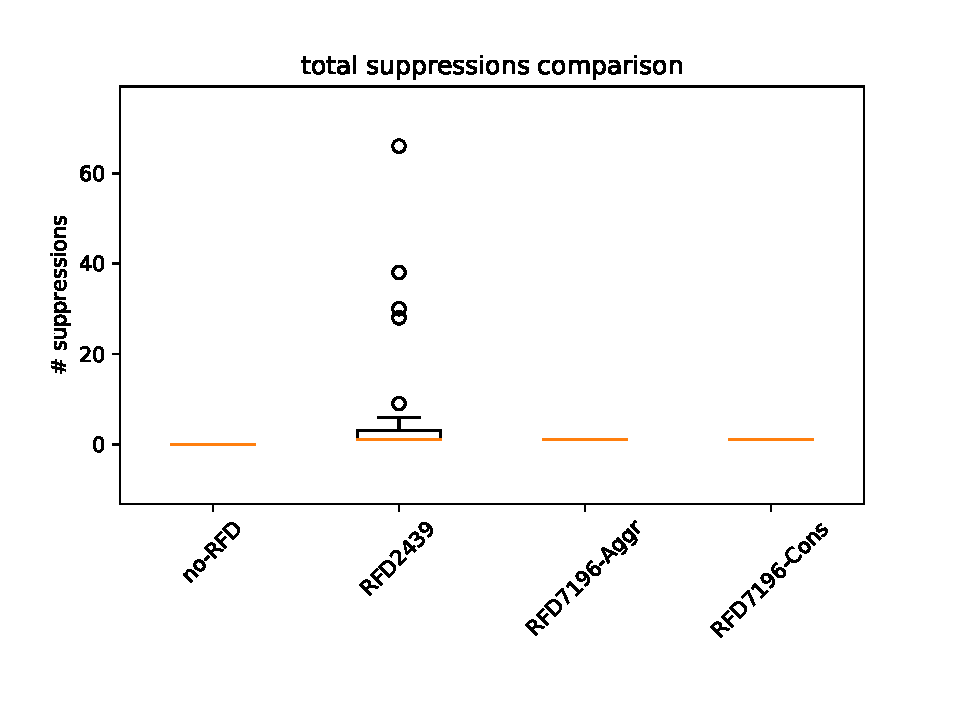
\includegraphics[width=\textwidth]{images/RFD/miceVSelephants/elephants/cisco_1000MRAI30_rfd_comparison_suppressions_boxplot.pdf}
%         \caption{Number of suppressions respect to the RFD strategy}
%         \label{fig:1000_RFD_MRAI_30_suppressions_elephant}
%     \end{subfigure}
%		\caption{Internet like topology \num{1000} nodes, \ac{MRAI} = \SI{30}{\second}, random destination, \num{100} flaps, \SI{3}{\second} delay, Network performances}
%        \label{fig:1000_RFD_MRAI_30_elephant}
%\end{figure}
%
%Is possible to see in \Cref{fig:1000_RFD_MRAI_30_elephant} that this time we have
%a different behaviour from all the \num{3} \ac{RFD} strategies.
%In \Cref{fig:1000_RFD_MRAI_30_suppressions_elephant} we can see that
%the standard strategy, on average, does more than \num{1250} suppression, producing
%the lowest number of messages, around \num{11000}, but the highest convergence
%time with more than \SI{5000}{\second}.
%All the suppression are trigger by the \textit{Path Exploration} problem that
%causes \ac{ADV} storms that trigger the suppression on the majority
%of the nodes.
%The two new strategies would produce on average just a few suppression in respect
%of the legacy one, but the number of messages doesn't differ too much.
%While there is a huge improvement on the convergence time, on average,
%both the new strategy permits the network to converge in less than \SI{4000}{\second}.
%All three strategy produce $1/3$ of the messages produced by the
%\textit{NoRFD} strategy.
%
%\begin{figure}[h]
%     \centering
%     \begin{subfigure}[b]{0.325\textwidth}
%         \centering
%         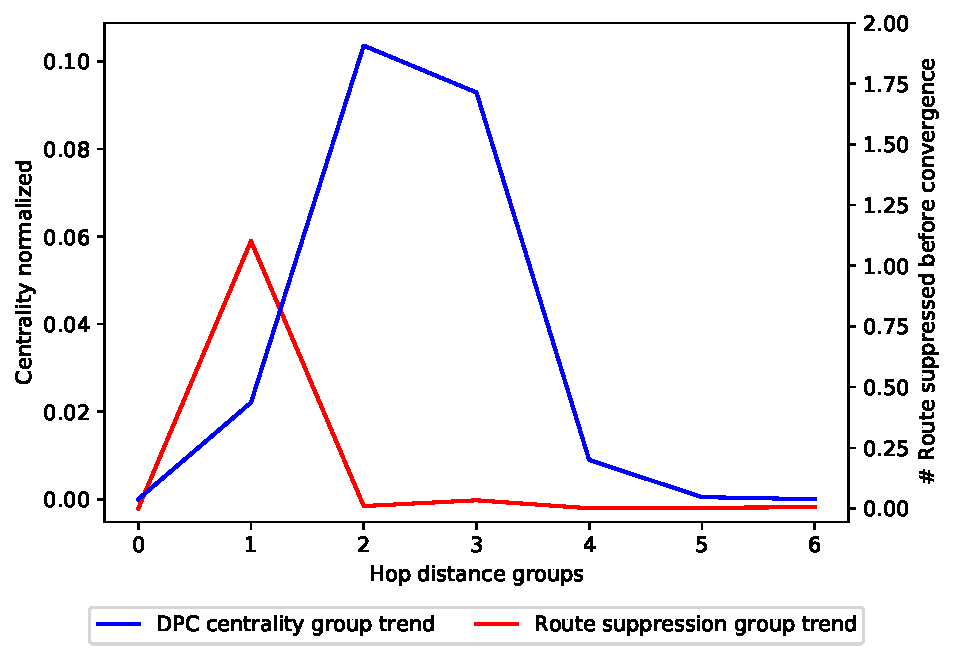
\includegraphics[width=\textwidth]{images/RFD/miceVSelephants/elephants/cisco_1000_RFD_nodeConvergence_centVSsup_trend.pdf}
%         \caption{RFD 2439 Strategy}
%         \label{fig:1000_2439RFD_cent_VS_sup_elephants}
%     \end{subfigure}
%     \hfill
%     \begin{subfigure}[b]{0.325\textwidth}
%         \centering
%         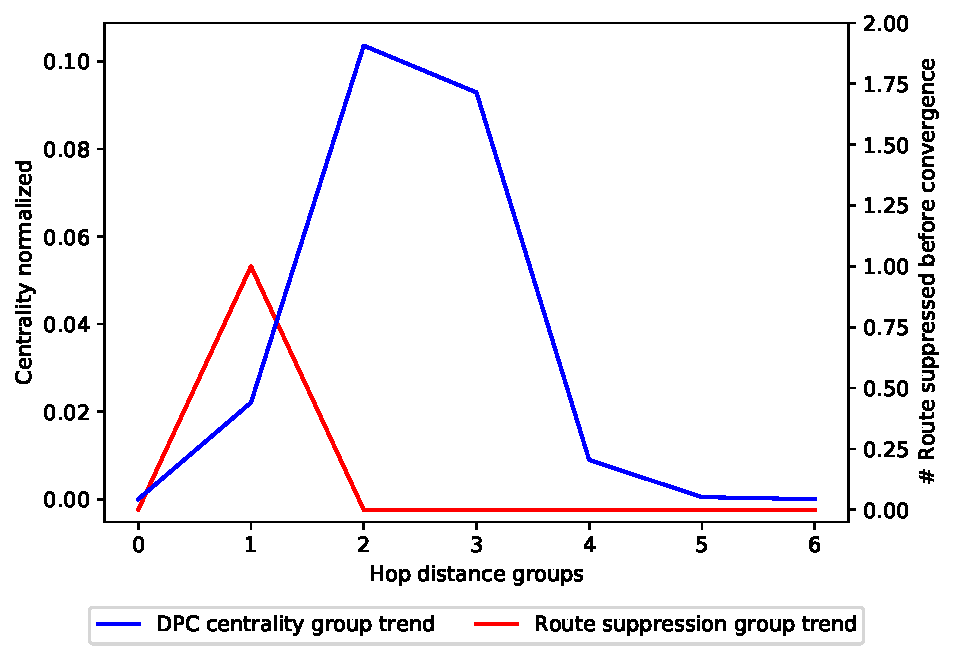
\includegraphics[width=\textwidth]{images/RFD/miceVSelephants/elephants/cisco_1000_RFD_7196_aggressive_nodeConvergence_centVSsup_trend.pdf}
%         \caption{RFD 7196 Aggressive Strategy}
%         \label{fig:1000_7196RFDA_cent_VS_sup_elephants}
%     \end{subfigure}
%     \hfill
%     \begin{subfigure}[b]{0.325\textwidth}
%         \centering
%         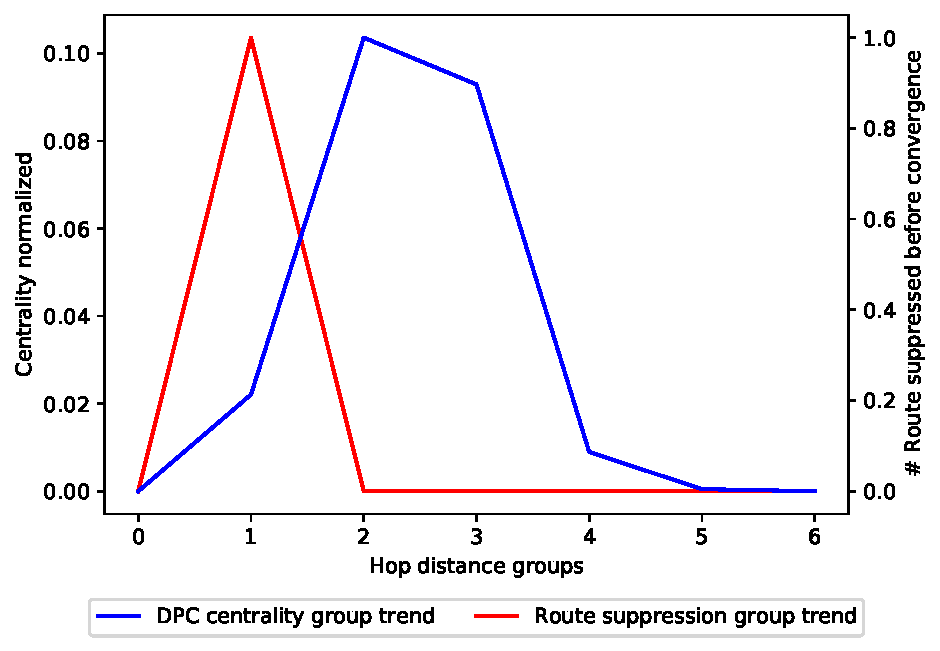
\includegraphics[width=\textwidth]{images/RFD/miceVSelephants/elephants/cisco_1000_RFD_7196_conservative_nodeConvergence_centVSsup_trend.pdf}
%         \caption{RFD 7196 Conservative Strategy}
%         \label{fig:1000_7196RFDC_cent_VS_sup_elephants}
%     \end{subfigure}
%		\caption{Internet like topology \num{1000} nodes, \ac{MRAI} = \SI{30}{\second},
%		random destination, \num{100} flaps, \SI{3}{\second} delay, suppressions
%		by distance from the source}
%        \label{fig:1000_RFD_cent_VS_sup_elephants}
%\end{figure}
%
%We can see in \Cref{fig:1000_RFD_cent_VS_sup_elephants} the comparison between
%the average number of suppressions per node group of the different strategies.
%In \Cref{fig:1000_7196RFDA_cent_VS_sup_elephants,fig:1000_7196RFDC_cent_VS_sup_elephants}
%we can notice that both strategies reacts in the exact same way at the elephant
%environment.
%The only nodes that suppress the route are the nodes that are closer to the source.
%All the other nodes of the network don't experience enough messages to block
%the route.
%In the first figure, \Cref{fig:1000_2439RFD_cent_VS_sup_elephants}, we can see
%that, on average, every node suppress at least one time the source of the
%signal.
%The hypothesis behind this trend is that the intervention of the closer nodes
%is not timely enough and all the other nodes have the time to experience the
%\textit{Path exploration} problem.
%With a lower threshold is sufficient a small number of \ac{ADV} storms
%to trigger the \ac{RFD} suppression.
%
%%We can then say that all the strategies catch in time the flap and avoid the
%%propagation of the update storm, increasing the convergence time but protecting
%%the network from thousands of messages.
%We can say that all the strategies protect the network from a huge load of messages.
%In \Cref{fig:1000_RFD_MRAI_30_messages_elephant} we can see that the use of \ac{RFD}
%reduces to $1/3$ the number of messages necessary to reach convergence.
%The difference is the convergence time, more nodes experience suppression
%then more time is necessary to converge because there will be more \ac{ADV} when
%the figure of merit becomes lower enough to activate again the route.
%For this reason there is a difference of more than \SI{1000}{\second} between
%the different techniques.
%This experiments reinforce the hypothesis that a small number of suppressions is
%more significant in respect of thousands of them.

\section{MRAI influence on Mice and Elephants}
\label{sec:bgp_rfd_mrai_influence_mice_elephants}

We can now study the influence of \ac{MRAI} on the \textit{Mice} and \textit{Elephants}
case.
The first one describes an environment with few flaps delayed in time, while the
second represent the opposite case with multiple flaps transmitted with high
frequency.
For this experiments I used the same environment described in \Cref{sec:rfd_mice_vs_elephants}.
The results of the \textit{Mice} case are exposed in \Cref{fig:1000_RFD_multiMRAI_mice},
while the results of the \textit{Elephants} case are presented in \Cref{fig:1000_RFD_multiMRAI_elephants}.

\begin{figure}[h]
     \centering
     \begin{subfigure}[b]{0.49\textwidth}
         \centering
         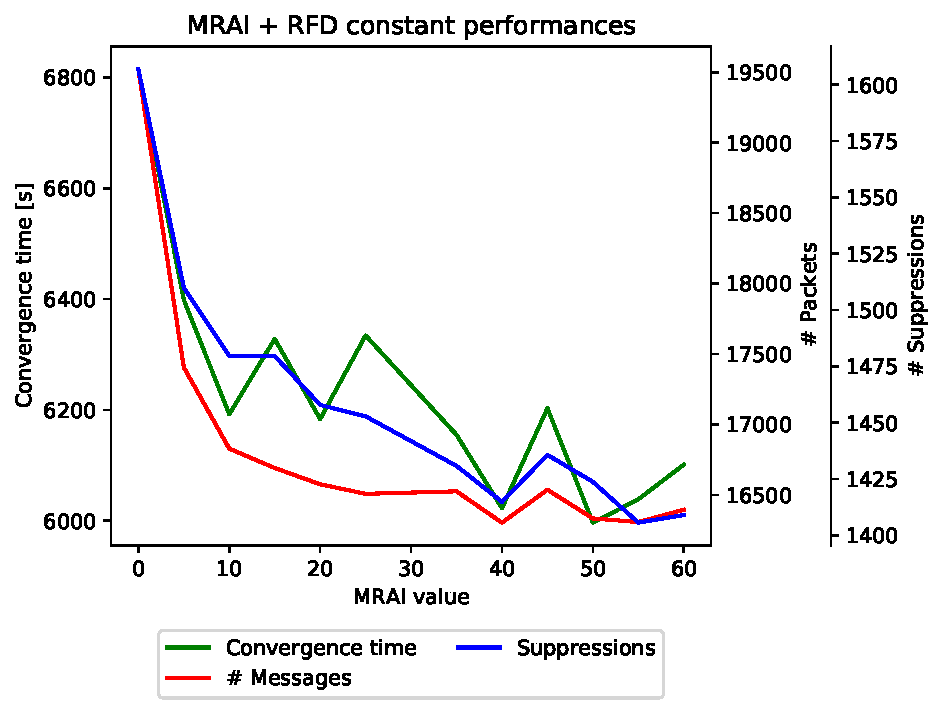
\includegraphics[width=\textwidth]{images/RFD/miceVSelephants/MultiMRAI/mice/cisco_1000_RFD_2439-constant_mrai_rfd_evolution.pdf}
         \caption{RFD 2439 Strategy}
         \label{fig:1000_2439RFD_multiMRAI_mice}
     \end{subfigure}
     \hfill
     \begin{subfigure}[b]{0.49\textwidth}
         \centering
         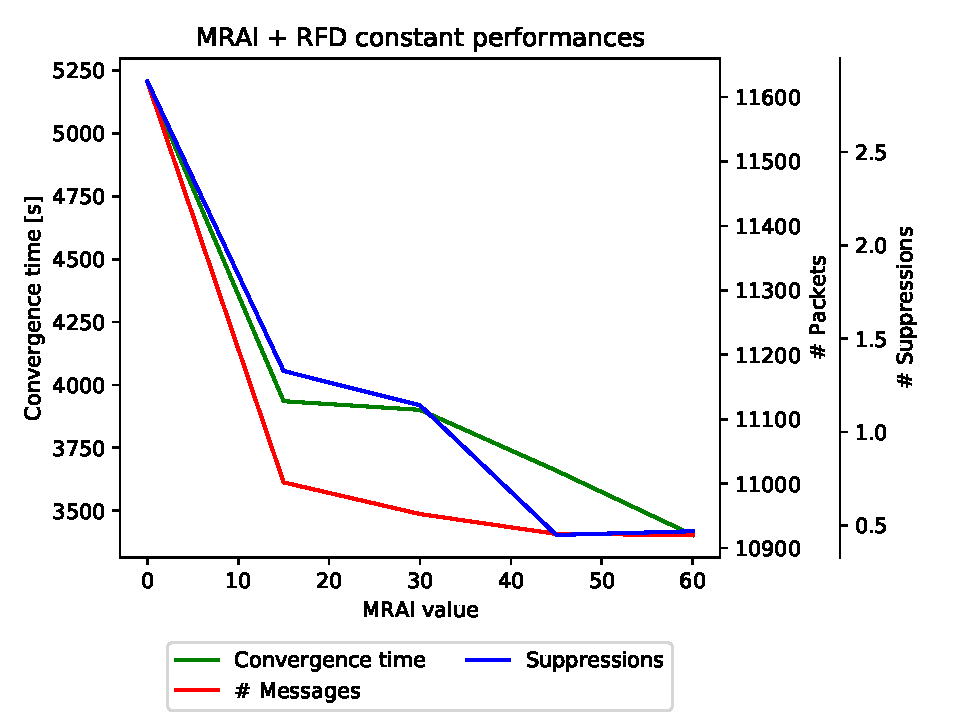
\includegraphics[width=\textwidth]{images/RFD/miceVSelephants/MultiMRAI/mice/cisco_1000_RFD_7196_aggressive-constant_mrai_rfd_evolution.pdf}
         \caption{RFD 7196 Aggressive Strategy}
         \label{fig:1000_7196RFDA_multiMRAI_mice}
     \end{subfigure}
     \begin{subfigure}[b]{0.49\textwidth}
         \centering
         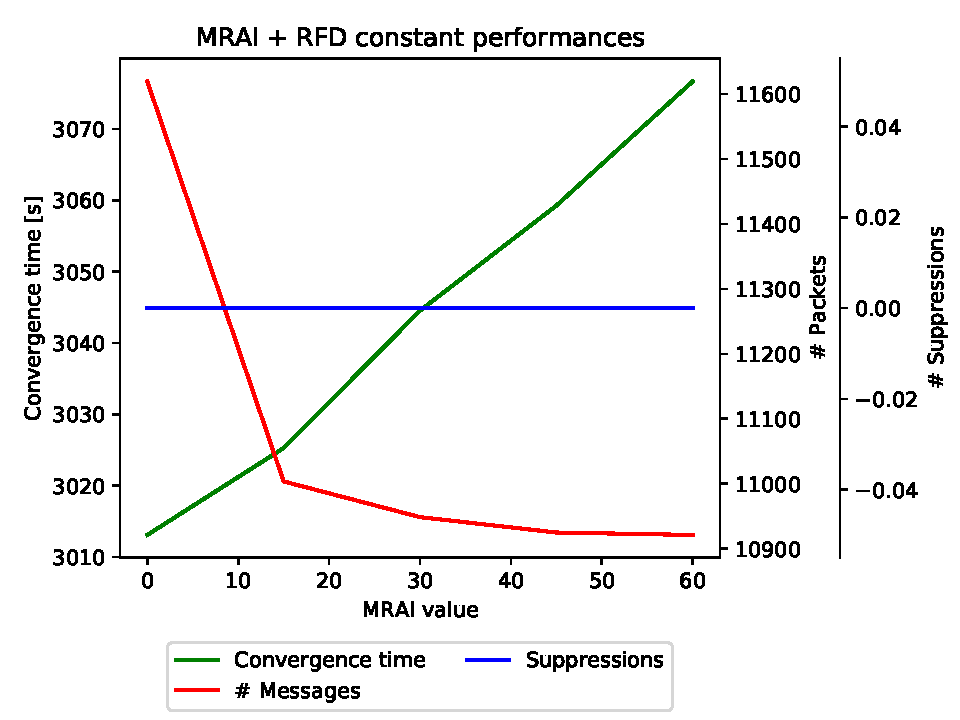
\includegraphics[width=\textwidth]{images/RFD/miceVSelephants/MultiMRAI/mice/cisco_1000_RFD_7196_conservative-constant_mrai_rfd_evolution.pdf}
         \caption{RFD 7196 Conservative Strategy}
         \label{fig:1000_7196RFDC_multiMRAI_mice}
     \end{subfigure}
		\caption{Internet like topology \num{1000} nodes, random destination,
		\num{5} flaps, \SI{300}{\second} delay, Network performances, \ac{MRAI}
		strategy fixed, \fxfatal{Adapt y ranges}}
        \label{fig:1000_RFD_multiMRAI_mice}
\end{figure}

\fxfatal{Redo this graphs with more \ac{MRAI} values, update the figures with the same y-range}

We can see in \Cref{fig:1000_RFD_multiMRAI_mice} how the different \ac{RFD} strategies
react, on the same topology, with different \ac{MRAI} settings.
The network performances with the legacy \ac{RFD} strategy from the \ac{RFC}
\num{2439} \cite{rfc2439} are presented in \Cref{fig:1000_2439RFD_multiMRAI_mice}.
First of all, is possible to see the influence of \ac{MRAI} on the number of suppressions
that decrease from \num{1600} with an \ac{MRAI} equal to \SI{0}{\second} to almost
\num{1400} with \ac{MRAI} $=$ \SI{60}{\second}.
The messaging trend reacts as expected with the increasing of
\ac{MRAI}, but, is remarkable that with an \ac{MRAI} of \SI{0}{\second} there
are less than \num{20000} messages thanks to \ac{RFD}.
The convergence time doesn't have the same trend as other \ac{MRAI} experiments,
it has a decreasing trend, while we were expecting an increasing one.
This is caused by the routes that don't suppress anymore the route.
It is greater the gain obtained by the suppression reduction than the disadvantage
caused by \ac{MRAI} that requires the nodes to wait more time.

The second case we can analyze is the \textit{Aggressive} strategy presented
in \Cref{fig:1000_7196RFDA_multiMRAI_mice}.
We can easily notice that this time the variation in terms of suppression is smaller,
going from a value of \num{1265} to \num{1240} suppressions.
The number of messages has a similar trend to the standard strategy, but with
a different range.
At the beginning, with \ac{MRAI} $=$ \SI{0}{\second} there are more than \num{42000}
messages, after a while it converges around a value of \num{37000} messages.
The convergence time respect the expected trend by the growth of \ac{MRAI}.
The higher number of messages is caused by the fact that \ac{RFD} requires more time
to activate itself, and in the meanwhile, a lot of messages storm will pass the
network.
The convergence time, in this case, is not affected by the decrease in the number
of suppressions.
The gain obtained by the \ac{RFD} suppression trend doesn't compensate the
effects of \ac{MRAI} that makes the convergence time grow.

In the last strategy, the \textit{Conservative} one, we can see another, different,
behaviour.
In terms of suppressions \ac{MRAI} makes a huge difference, we go from \num{1200}
suppressions to \num{0}, is sufficient an \ac{MRAI} of \SI{15}{\second} to reduce
it around \num{50}.
Also in this case, the number of messages is higher than the other two strategies.
The higher suppression threshold, like for the \textit{Aggressive} strategy, permits
multiple \ac{ADV} storms without blocking the route.
An interesting behaviour can be seen for the convergence time, in fact like for
the \textit{Aggressive} strategy it starts growing also with more than \num{1000}
suppressions of difference, but as soon the number of suppression touches \num{0}
it goes back to the \textit{NoRFD} behaviour.

Multiple comparison, with different \ac{MRAI} value can be also seen in
\Cref{fig:1000_RFD_MRAI30_mice}.
In \Cref{fig:1000_RFD_centVSsup_mices} is also possible to see how the different
\ac{MRAI} values modify the suppression behaviour in relation of the position of
the node in the network.

In \Cref{fig:1000_RFD_multiMRAI_elephants} are presented the results obtained
with the elephant environment and multiple \ac{MRAI} values.

\begin{figure}[h]
     \centering
     \begin{subfigure}[b]{0.49\textwidth}
         \centering
         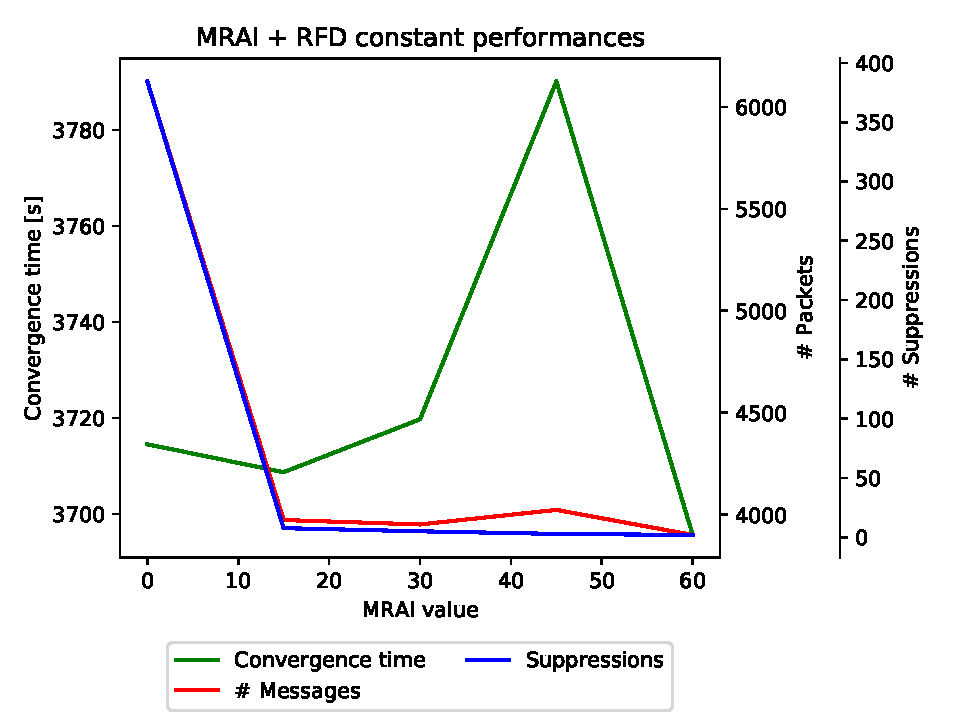
\includegraphics[width=\textwidth]{images/RFD/miceVSelephants/MultiMRAI/elephants/cisco_1000_RFD_2439-constant_mrai_rfd_evolution.pdf}
         \caption{RFD 2439 Strategy}
         \label{fig:1000_2439RFD_multiMRAI_elephants}
     \end{subfigure}
     \hfill
     \begin{subfigure}[b]{0.49\textwidth}
         \centering
         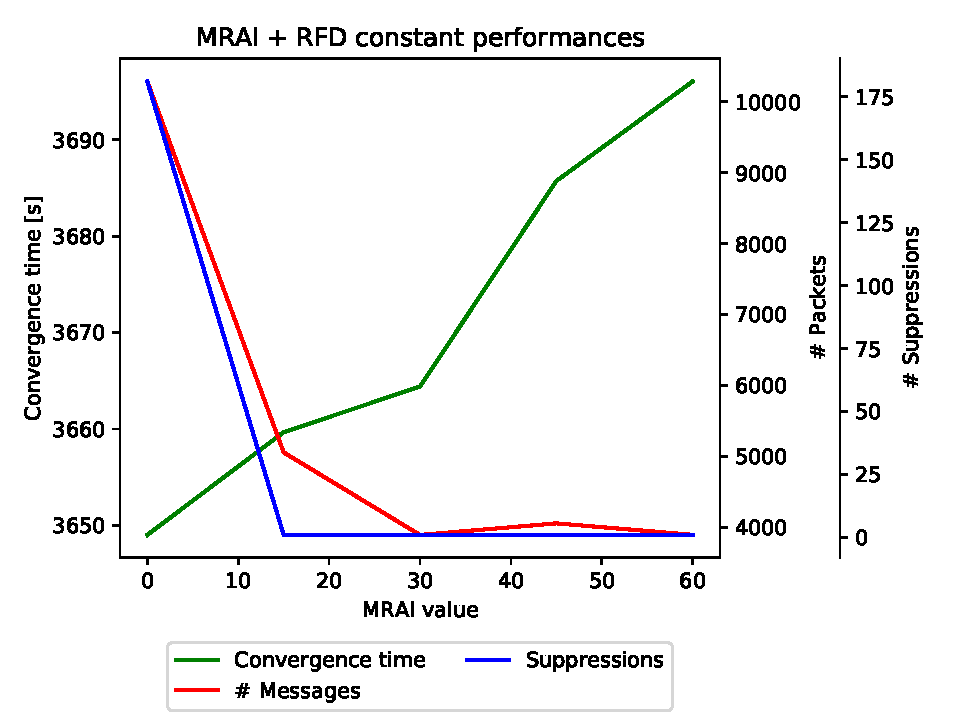
\includegraphics[width=\textwidth]{images/RFD/miceVSelephants/MultiMRAI/elephants/cisco_1000_RFD_7196_aggressive-constant_mrai_rfd_evolution.pdf}
         \caption{RFD 7196 Aggressive Strategy}
         \label{fig:1000_7196RFDA_multiMRAI_elephants}
     \end{subfigure}
     \begin{subfigure}[b]{0.49\textwidth}
         \centering
         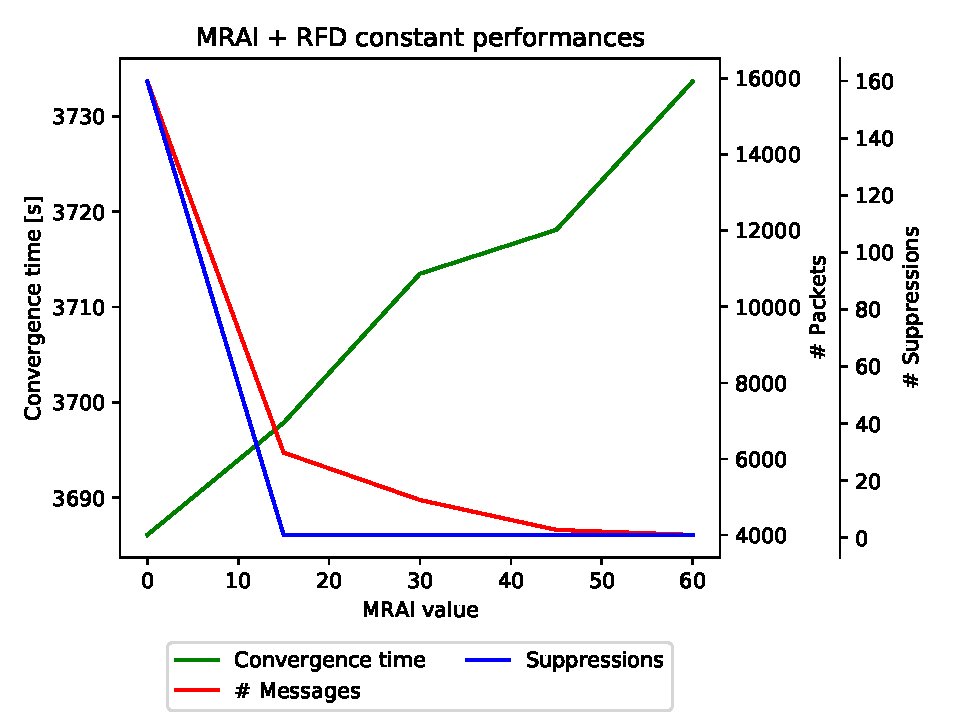
\includegraphics[width=\textwidth]{images/RFD/miceVSelephants/MultiMRAI/elephants/cisco_1000_RFD_7196_conservative-constant_mrai_rfd_evolution.pdf}
         \caption{RFD 7196 Conservative Strategy}
         \label{fig:1000_7196RFDC_multiMRAI_elephants}
     \end{subfigure}
		\caption{Internet like topology \num{1000} nodes, random destination, \num{100} flaps, \SI{3}{\second} delay, Network performances}
        \label{fig:1000_RFD_multiMRAI_elephants}
\end{figure}

The trends in the elephant case are completely different in respect to the
mice environment.
Starting from the standard strategy in \Cref{fig:1000_2439RFD_multiMRAI_mice}
we can see that the number of suppression decreases of a few hundred units
thanks to a higher \ac{MRAI}.
Also, the number of messages decrease from around \num{14500} reaching a stable
state around \num{11000}.
While the convergence time benefits of the suppression rate decrease, reaching
a valley around \SI{5400}{\second}.
But, after that point, the effect of avoiding the next suppression set is not enough to keep
a descending trend, while \ac{MRAI} acquire a more predominant position making
the convergence time slightly increasing.

A different behaviour can be saw in
\Cref{fig:1000_7196RFDA_multiMRAI_elephants,fig:1000_7196RFDC_multiMRAI_elephants},
where the number off suppression, thanks to \ac{MRAI}, reaches a number slightly
higher than \num{0}.
The number of messages reaches the same convergence point around \num{12500} but
with a completely different starting point.
With \ac{MRAI} at \SI{0}{\second} the aggressive strategy presents a number of
messages around \num{32500} while the conservative strategy is around \num{60000},
almost the double of the \textit{Aggressive} one.
This huge difference is caused by the fact that the \textit{conservative} strategy requires
more flaps to overcome the suppression threshold, and all those messages can
cause more and more updates storms due to the \textit{Path exploration} problem
in other parts of the network.
In both, \textit{Aggressive} and \textit{Conservative} strategy, the convergence
time is not affected by the variation on the number of suppressions but it's only
affected by the growth of \ac{MRAI}.

The fact that in the last two strategies the time is not affected by the huge number
of suppression could be saw as an error, but it is not.
In fact, the suppressions with an \ac{MRAI} of \SI{0}{\second} happens
few seconds after the beginning of the experiment and the majority of the nodes
will suppress the route, but we know that after \SI{3600}{\second} a route
can't be suppressed anymore.
For this reason after that time, there will be just a last update storm to propagate
the reintroduction of the route.
And, on average, all the nodes will converge a few seconds after \SI{1}{\hour}.
Causing \ac{MRAI} to be the only influence factor after \SI{1}{\hour}.

We can then conclude that \ac{MRAI} influences both the \textit{Mice} and
\textit{Elephants} cases.
The major effects can be saw on the two modern strategies of \ac{RFD}.
For the \textit{Mice} environment, those two strategies will tend to have
a behaviour similar to the \textit{NoRFD} strategy. And \ac{MRAI} would
influence the number of suppressions and indirectly the convergence time
and the number of messages transmitted.
We can see from \Cref{fig:1000_RFD_centVSsup_mices} that also the set of
nodes that triggers the suppressions change.
We can see even more effects in the \textit{Elephants} environment, where
\ac{MRAI} highly impact the number of suppressions.
Both the \textit{Aggressive} and \textit{Conservative} strategies would present
just few suppression in comparison of the thousands suppression triggered with the
legacy \num{2439} strategies.
And the new strategies would have a high impact on the convergence time, at
the cost of a few hundred messages on average.
In \Cref{fig:1000_RFD_centVSsup_elephants} is possible to see the effects
on the set of nodes that effectively suppress the route, in the legacy
case even the more distance nodes would suppress it, while with the new
strategies is sufficient a suppression near the source, and \ac{MRAI} would
help to prevent suppressions due to the \textit{Path exploration} problem.

This is an other confirm that \ac{MRAI} is fundamental for the sustainability of
Internet, while \ac{RFD} have a more marginal impact.

%\begin{itemize}
%    \item What is Mice VS Elephants?
%    \item How has been studied in the past?
%    \item Introduce how MRAI affects mice VS elephants
%\end{itemize}
